\documentclass[aps, jcp, prl, reprint, groupedaddress, superscriptaddress, twocolumn]{revtex4-1} 
%\usepackage{graphicx,topcapt,booktabs,hyperref,url, float,multirow,caption,subcaption,bm}
\usepackage{graphicx, color, bm, amsmath, multirow, subcaption, topcapt, hyperref}
\usepackage[ labelfont=bf, font = small, justification=justified, format=plain]{caption}


\begin{document}

\title{A Single-Site Model for Water: Parameterized for the Reproduction of the Melting Point of Ice I$_h$}
\author{Patrick B. Louden}
\author{J. Daniel Gezelter}
\affiliation{Department of Chemistry, University of Notre Dame, Notre Dame, IN 46556}

%macros
\newcommand{\degree}{\ensuremath{^\circ}}

\begin{abstract}
This report is a living document on the progress of developing a single-site
model for water, parameterized to reproduce the experimentally observed
melting point of ice I$_h$.
\end{abstract}

\maketitle


\section{Introduction}
Abascal and Vega have recently observed that the melting points of common 
3-site and 4-site water models correlates strongly with their dipolar and 
quadrupolar interactions.\cite{Abascal07b,Abascal07c,Abascal07d} To quantify
dipole and quadrupole moments, we must first consider how to define our
coordinate system. For planar
water models, we define our coordinate system in the following way;
the $z$ axis as the dipole moment direction (the HOH bisector), the $y$ axis
parrallel to the vector connecting the two Hydrogens, and the $x$ axis normal 
to the plane of the molecule. This choice of coordinate system follows that of
Rick, and thus the equations in his paper follows naturally. 
Abascal and Vega define their coordinate system by flipping the $x$ and $y$
axes, resulting in a few sign changes between our work and theirs. Having 
defined a coordinate system, we can calculate the traceless quadrupole tensor,
$\Theta$, for any water model by

\begin{equation}
\Theta_{ij} = \frac{1}{2} \sum_{\alpha}q_{\alpha}(3r_{i,\alpha}r_{j,\alpha}-|\vec{r_{\alpha}}|^{2}\delta_{ij})
\end{equation}

where, $q$ is the charge and the sum is taken over all charged sites in the 
model. The traceless quadrupole tensor has certain special properties, and
is aptly named for one of them; which is the trace, ($Tr$), of the tensor 
is null.

\begin{equation}
Tr(\Theta) = \sum_{i,j}\Theta_{ij}\delta_{ij} = 0
\end{equation}

While having a traceless tensor can make certain calculations easier to 
perform, it is also possible to calculate a traced quadrupole tensor $Q$, one
in which the trace is not null.

\begin{equation}
Q_{ij} = \frac{1}{2}\sum_{\alpha}q_{\alpha}(r_{i,\alpha}-r_{i,com})(r_{j,\alpha}-r_{j,com})
\end{equation}

Here, $r_{i,com}$ is the position of the center of mass in the $i$-th 
dimension, and therefore the position of the quadrupole moment is set at the 
center of mass of the molecule. It will be desirable to change between the
traceless and traced quadrupole tensors during this work, and changing 
between the two formalisms can be achieved by the following

\begin{equation}
\Theta = 3Q - Tr(Q)
\end{equation}    

Based on the suggestion of Carnie and Patey\cite{Carnie82}, 
as well as Rick\cite{Rick04}, Abascal and Vega have described an effective 
tetrahedral quadrupole moment ($\Theta_T$), defined in ours and Rick's 
coordinate 
system for a traceless quadrupole as

\begin{equation}
\Theta_{T} = \frac{1}{2}(\Theta_{yy} - \Theta_{xx}).
\end{equation} 

Abascal and Vega have shown that the water models which most accurately
reproduce the meling point of ice I$_h$ have a ratio of their dipole moment
to $\Theta_T$ of approximately unity. The equivalent expression for the 
traced quadrupole tensor is given as

\begin{equation}
Q_{T} = \frac{3}{2}(Q_{yy} - Q_{xx}).
\end{equation}
 
The Q$_T$ values for each of the water models
investigated by Abascal and Vega are shown in Table \ref{Models_quad}, along 
with the non-zero elements of their traced quadrupole tensors.

\begin{table}[h!]
\begin{tabular}{|c|c|c|c|c|c|c|c|}
\hline
& $Q_{xx}$ & $Q_{yy}$ & $Q_{zz}$ & $Tr(Q)$ & QBar & $Q_{T}$ & T$_{m}$ \\
\hline
TIP4P/Ice & 0.0 & 1.6629 & 0.7427 & 2.3657 & 2.8143 & 2.4348  & 272.2 \\
TIP4P/2005 & 0.0 & 1.531 & 0.7034 & 2.2336 & 2.6553 & 2.2969  & 252.1 \\
TIP4P/Ew & 0.0 & 1.4427 & 0.6617 & 2.1044  & 2.5017 & 2.1640  & 245.5   \\
TIP4P & 0.0 & 1.4311 & 0.6584 & 2.0895 & 2.4814 & 2.1466 & 232.0 \\
SPC/E & 0.0 & 1.357 & 0.5267 & 1.8837 & 2.3700 & 2.0356 & 215.0 \\
SPC & 0.0 & 1.3129 & 0.5095 & 1.8224 & 2.2928 & 1.9693 & 109.5 \\
TIP3P & 0.0 & 1.1476 & 0.5337 & 1.6812 & 1.9894 & 1.7214 & 146 \\
\hline
\end{tabular}
\caption{Traced quadrupole tensors for the water models investigated by Abasca and Vega. All elements of the tensors are in units of D\AA~, melting temperatures are reported in Kelvin.}
\label{Models_quad}
\end{table} 

In Figures \ref{fig:QBar} and \ref{fig:TraQ},
we have replotted the 
melting point for ice I$_h$ of these water models by $\overline{Q}$ and the 
trace of their
quadrupole tensor, where $\overline{Q}$ is given by,

\begin{equation}
\overline{Q} = \sqrt{2(3 Q:Q - (Tr(Q))^{2})}
\end{equation}

We see in both cases there is a strong correlation between
the values of their quadrupole tensors and their melting point.

\begin{figure}[h!]
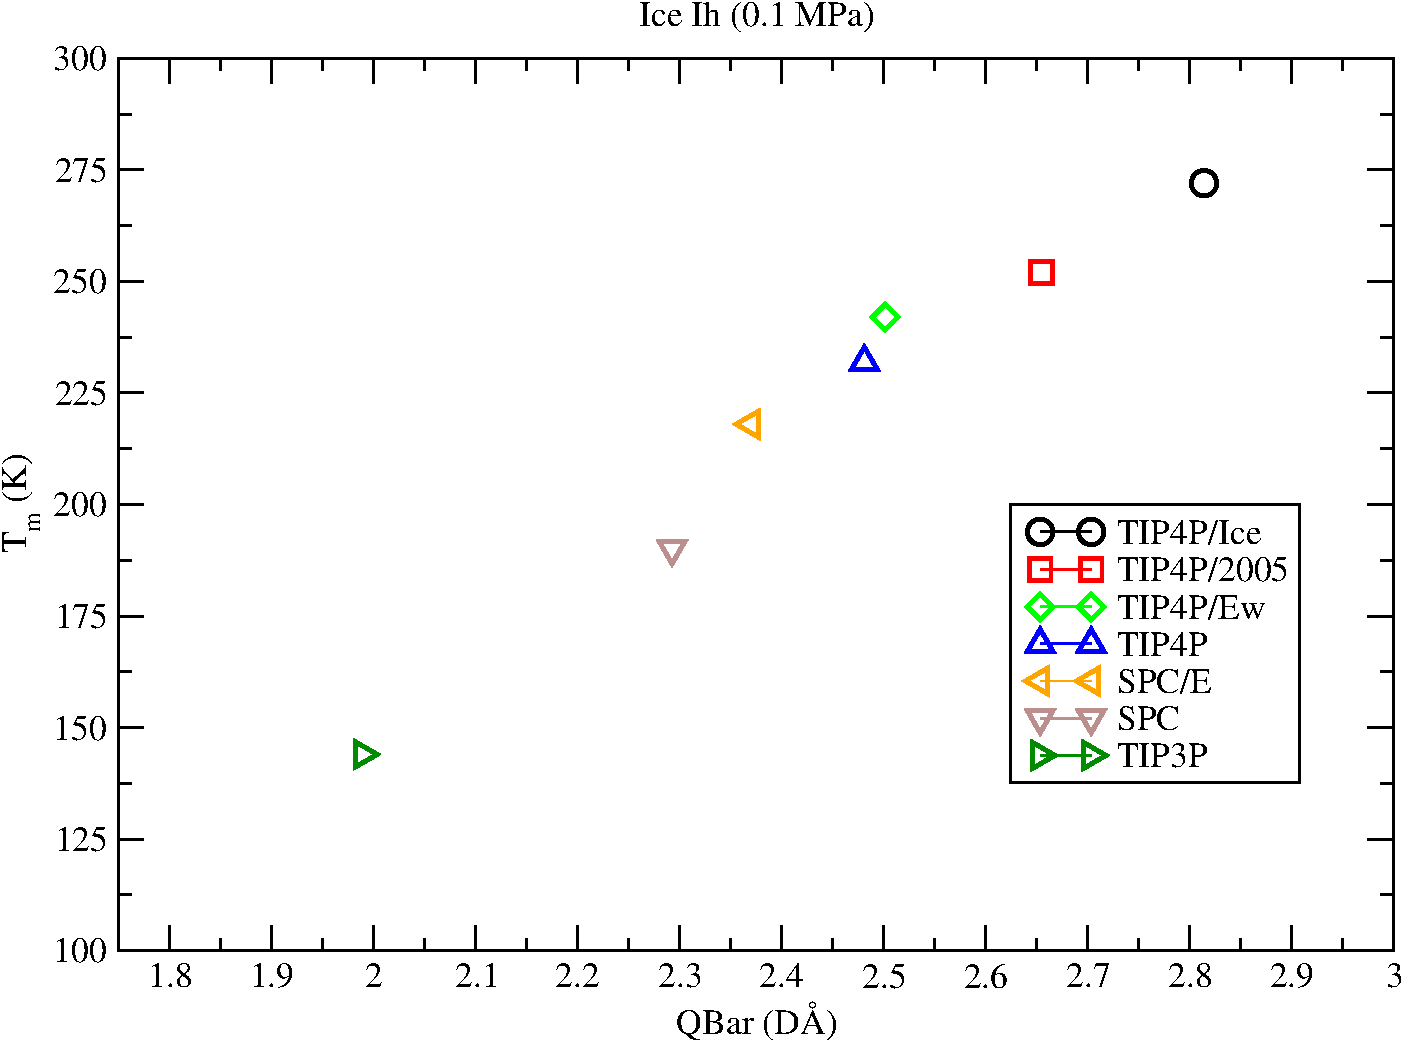
\includegraphics[width = 0.5\textwidth]{Tm_Ih_Qbar_plot.pdf}
\caption{\label{fig:QBar} Melting point for ice I$_h$ of several popular water models as a function of the QBar for the model. We see a strong correlation between a more accurate melting point and a larger value of QBar. We estimate that a QBar of approximately 2.8 D\AA will result in the experimental melting point of 273.15 K. A linear regression of the data resulted in an equation of best fit of $y = 158.89x - 166.83$. From this, we have predicted an optimal QBar to be 2.7690 D\AA~.}
\end{figure}

\begin{figure}[h!]
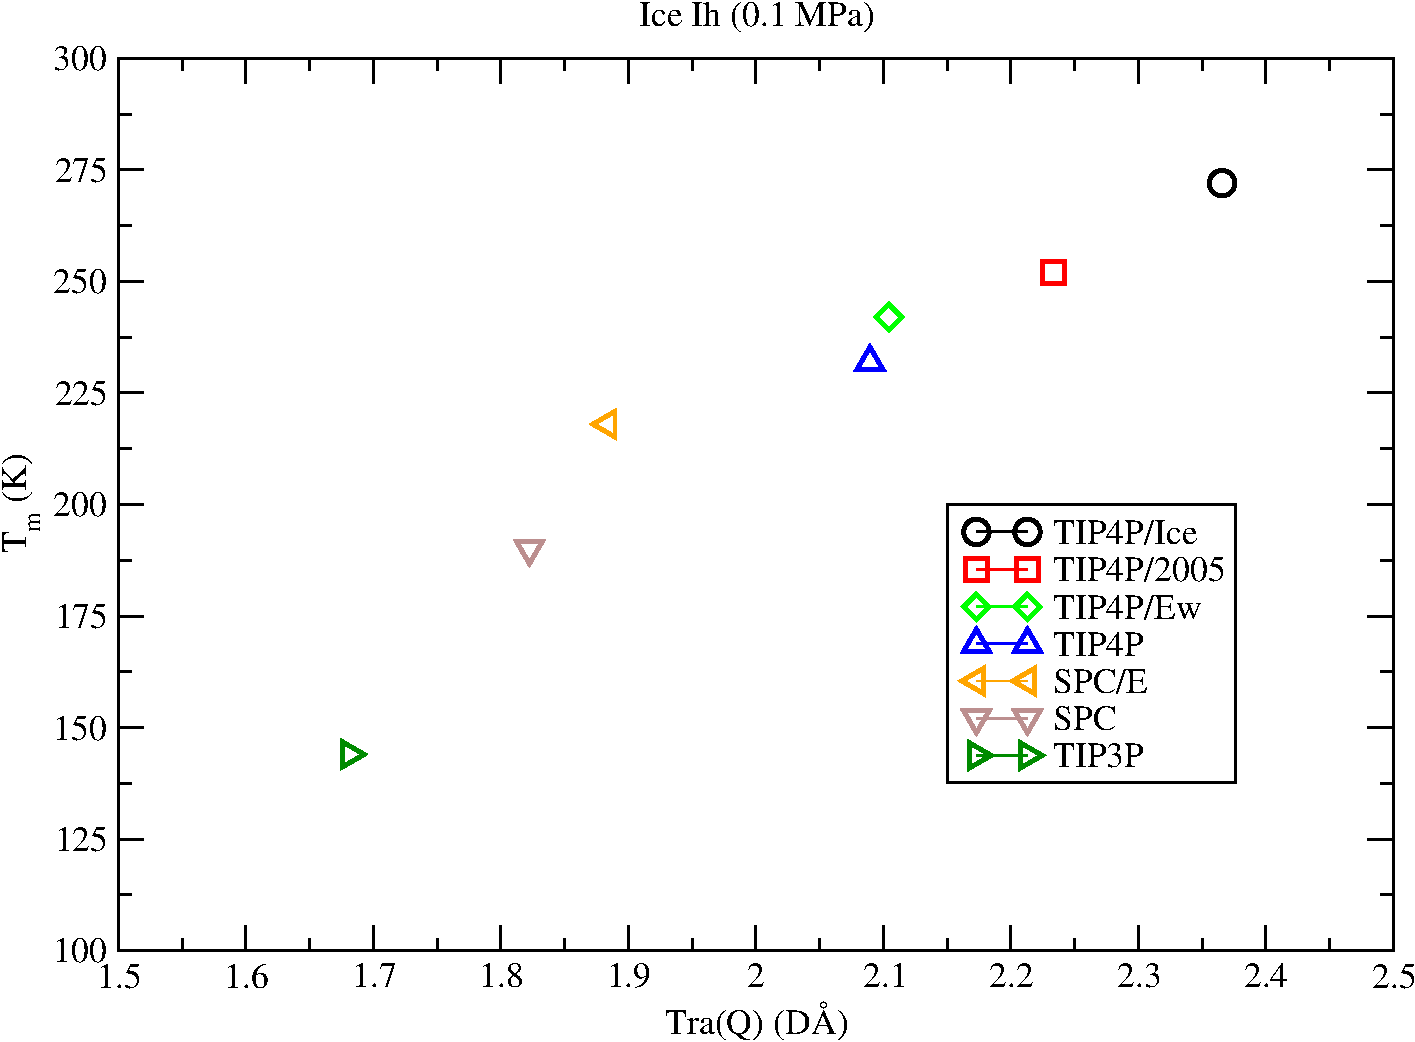
\includegraphics[width = 0.5\textwidth]{Tm_Ih_TraQ_plot.pdf}
\caption{\label{fig:TraQ} Melting point for ice I$_h$ of several popular water models as a function of the trace of the quadrupole tensor for the model. We see a strong correlation between a more accurate melting point and a larger value of the trace. We estimate that a trace of approximately 2.3 D\AA will result in the experimental melting point of 273.15 K.}
\end{figure}



Based on this observation, we have begun work on a 1-site model with intentions
of setting the dipole moment and structuring the quadrupole tensor in such
a way that will give us a ratio of unity. As a starting point, we have 
collapsed the 4-site TIP4P-Ice model\cite{Abascal05b} onto a 1-site model 
(TIP1P/Ice). The 
geometric parameters, the Lennard-Jones and charges, and the dipole and 
quadrupole elements that have value can be found for both models in 
Table \ref{Geo_Params}, Table \ref{LJq_Params}, and Table \ref{DQ_Params} 
respectively.

\begin{table}[h!]
\begin{tabular}{|c|c|c|c|}
\hline 
& OH bond length \AA & OM bond length \AA & HOH \degree\\
\hline 
TIP4P/Ice & 0.9572 & 0.1577 & 104.52 \\
TIP1P/Ice & - & - & - 			      \\
\hline
\end{tabular}
\caption{Geometric parameters of the TIP4P/Ice and TIP1P/Ice models.}
\label{Geo_Params}
\end{table}

\begin{table}[h!]
\begin{tabular}{|c|c|c|c|c|}
\hline
& $\sigma$ \AA & $\epsilon$ kcal/mol & q$_H$ (e) & q$_M$ (e) \\
\hline 
TIP4P/Ice & 3.1668 & 0.2108509 & 0.5897 & -1.1794 \\
TIP1P/Ice & 3.1668 & 0.2108509 & - & -            \\
\hline
\end{tabular}
\caption{Lennard-Jones and charge parameters of the TIP4P/Ice and TIP1P/Ice models.}
\label{LJq_Params}
\end{table}

\begin{table}[h!]
\begin{tabular} {|c|c|c|c|c|c|}
\hline
& $\mu$ D & Q$_{xx}$ D\AA & Q$_{yy}$ D\AA & Q$_{zz}$ D\AA & Q$_T$ D\AA \\
\hline
TIP4P/Ice & 2.4255966 & 0.0 & 1.62291807 & 0.74278997 & 2.434 \\
TIP1P/Ice & 2.4255966 &0.0 & 1.62291807 & 0.74278997 &2.434 \\
\hline
\end{tabular}
\caption{Dipole and quadrupole parameters for the TIP4P/Ice and TIP1P/Ice models.}
\label{DQ_Params}
\end{table}


\section{TIP1P/Ice}
\subsection{Gas Phase Dimer}
This section contains details and graphs of the attempts to tune the TIP1P/Ice
model to the experimental and ab initio predicted results for the gas phase
water dimer. In order to tune the TIP1P/Ice model, we are going to calculate 
the geometry of the gas phase water dimer as shown in Figure 
\ref{fig:dimer}\cite{Yu04}.

\begin{figure}[h!]
\includegraphics[width = 0.5\textwidth]{dimer.pdf}
\caption{\label{fig:dimer} The gas phase water dimer geometry.}
\end{figure}

There are three values of interest for our characterization of the water dimer.
The first is the oxygen-oxygen separation distance, R$_{OO}$. The other two
parameters of the dimer are the two angles, $\theta$ and $\phi$. These angles
are taken from the HOH bisector to the R$_{OO}$ vector. While the length
of the R$_{OO}$ vector will be dependent on the magnitude of the dipole and 
quadrupole moments, the relative contributions of Q$_{xx}$, Q$_{yy}$, and
Q$_{zz}$ will strongly influence the angles. We also expect that the 
Lennard-Jones parameter $\sigma$ will strongly influence the magnitude of
the R$_{OO}$ vector.
The experimentally measured and computationally predicted values for the 
geometry of the water
dimer can be found in Table \ref{dimer_geo}. Also in Table \ref{dimer_geo}, we
see the geometry parameters computed at 0.1 K for the TIP4P/Ice and TIP1P/Ice
models.

\begin{table}[h!]
\begin{tabular}{|c|c|c|c|}
\hline
& R$_{OO}$ (\AA) & $\theta$ (\degree)& $\phi$ (\degree) \\
\hline
Expt.     & 2.95 & 51 $\pm$ 10 & 57 $\pm$ 10 \\ 
Ab initio & 2.91 & 56    & 58    \\
TIP4P/Ice & 2.79 & 52.52 & 43.17 \\
TIP1P/Ice & 2.83 & 40.56 & 36.59 \\
\hline
\end{tabular}
\caption{Geometric parameters of the TIP4P/Ice and TIP1P/Ice gas phase water dimer. Ab initio and Expt. values were taken from another source\cite{Yu04}.}
\label{dimer_geo}
\end{table}

\subsubsection{Testing Electrostatic Cutoff}
First we will see if we can recover the TIP4P/Ice dimer geometry by decreasing
damping $\alpha$ to 0.05 \AA$^{-1}$ and vary the cutoff radius for the
electrostatics. In Figure \ref{fig:rcut}, we see that with very small damping 
$\alpha$, increasing the cutoff radius of the potential
does not recover the TIP4P/Ice calculated geometry.

\begin{figure}[h!]
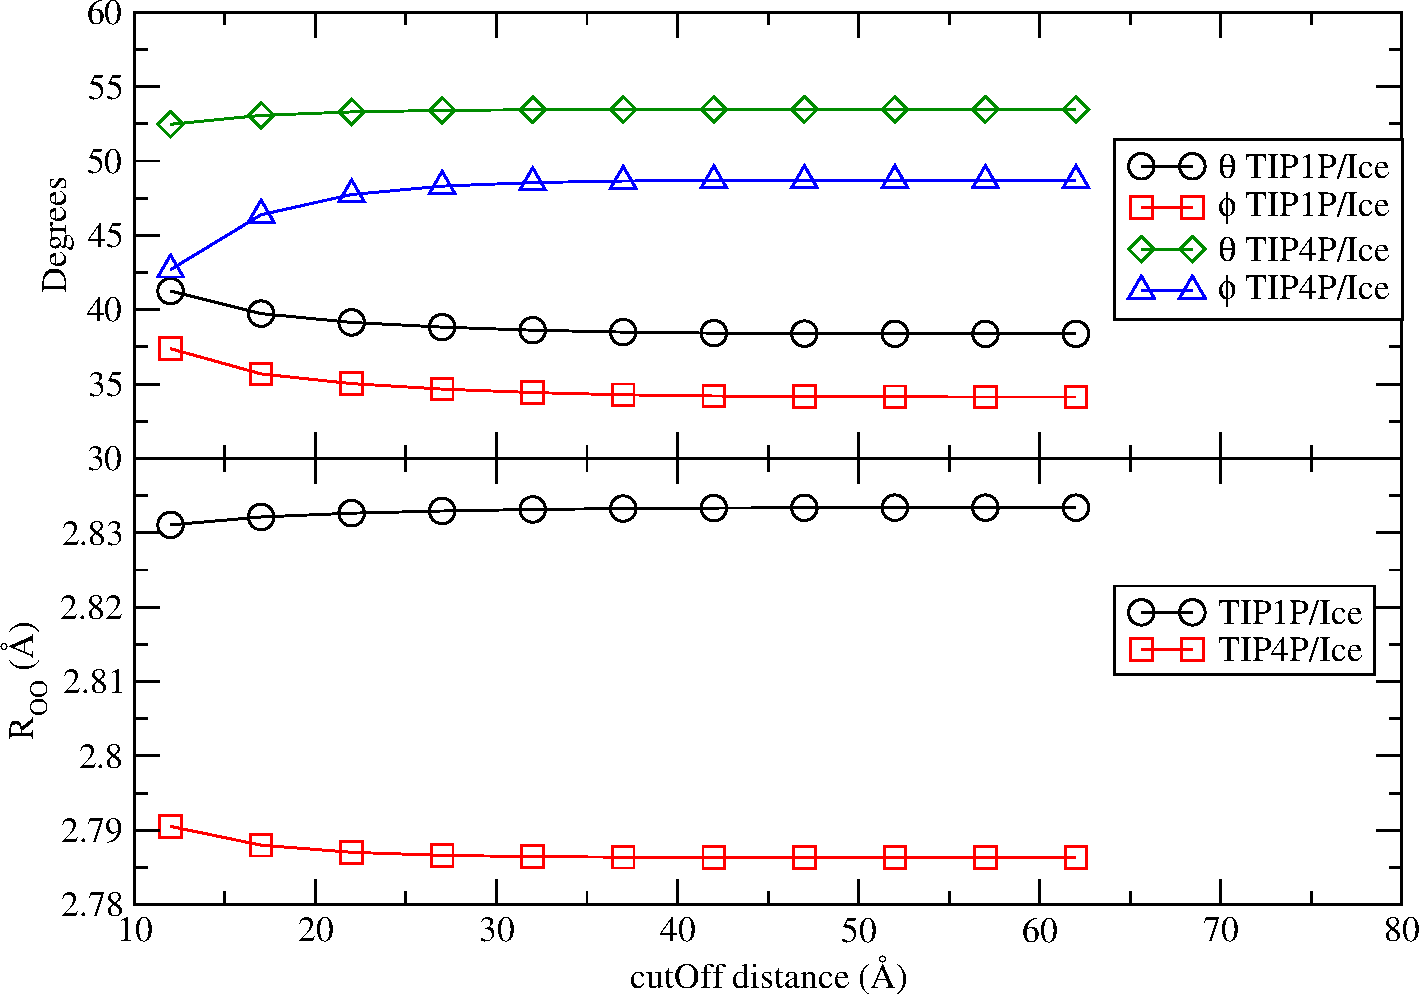
\includegraphics[width = 0.5\textwidth]{Test17_plot.pdf}
\caption{\label{fig:rcut} Damping $\alpha$ set to 0.05 \AA$^{-1}$ and the simulation box was $300\times300\times300$ \AA~.}
\end{figure}

\subsubsection{Varying Lennard-Jones Parameters}
In our initial test, as seen in Figure \ref{fig:Sigma}, the Lennard-Jones 
parameter $\sigma$ was varied 
while holding the other parameters of the TIP1P/Ice model constant. We see that
the ab. initio predicted R$_{OO}$ separation distance of 2.91 \AA is obtained
when $\sigma$ is set to approximately 3.25 \AA . However, the two angles 
$\theta$ and $\phi$ tend to decrease with increasing values of $\sigma$, 
and result in values of about 36\degree and 31\degree, which is in poor 
agreement with the ab. initio calculations. Also, changing the Lennard-Jones
parameter $\sigma$ will drastically alter the condensed phase properties
of the model. Namely, the radial distribution function is very sensative to
$\sigma$. The location of the first solvation shell can be tuned by $\sigma$,
so we will initially retain the TIP4P/Ice model's value of 3.1668 \AA~ and vary
it later if the radial distribution function is off.


\begin{figure}[h!]
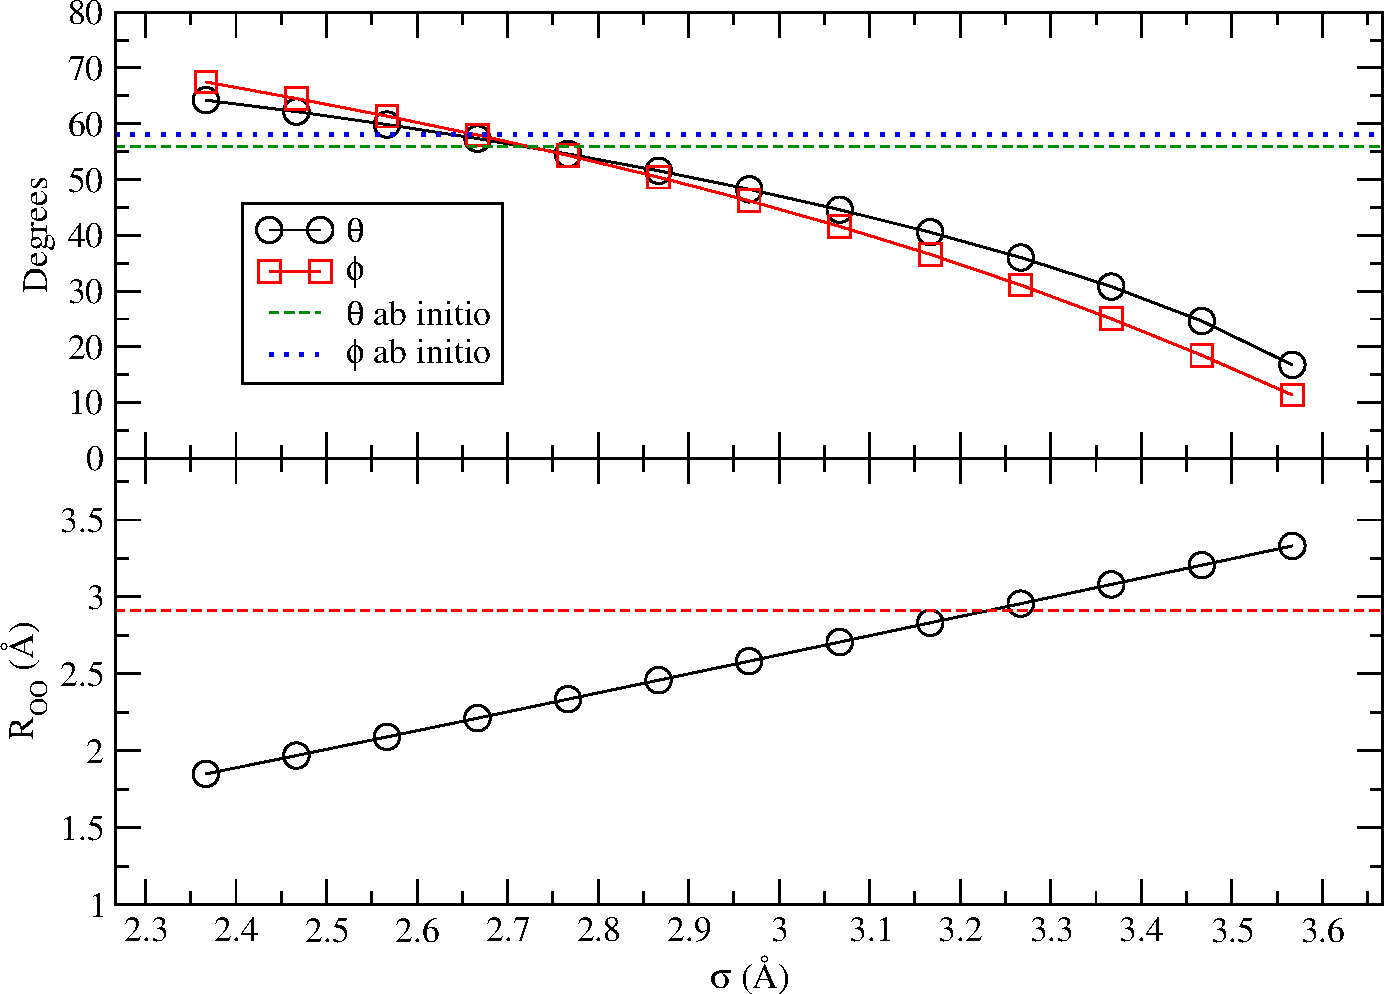
\includegraphics[width = 0.5\textwidth]{Test1_plot.pdf}
\caption{\label{fig:Sigma} The Lennard-Jones parameter $\sigma$ was varied while holding the other parameters of the TIP1P/Ice model constant.}
\end{figure}


Next, we will vary the Lennard-Jones parameter $\epsilon$, as seen in 
Figure \ref{fig:Epsilon}. We see that the ab. initio calculated value 
of R$_{OO}$ 
distance of about 2.91 \AA is achieved when $\epsilon$ is set to 
approximately 0.275 kcal/mol. However, both $\theta$ and $\phi$ tend to 
decrease with increasing $\epsilon$, and the resulting values for the two 
angles at this value of $\epsilon$ are approximately 38\degree and 33\degree,
which are again far from the predicted values. Changing $\epsilon$ is not a
great way to parameterize the model though, and we will avoid doing so as much
as possible.

\begin{figure}[h!]
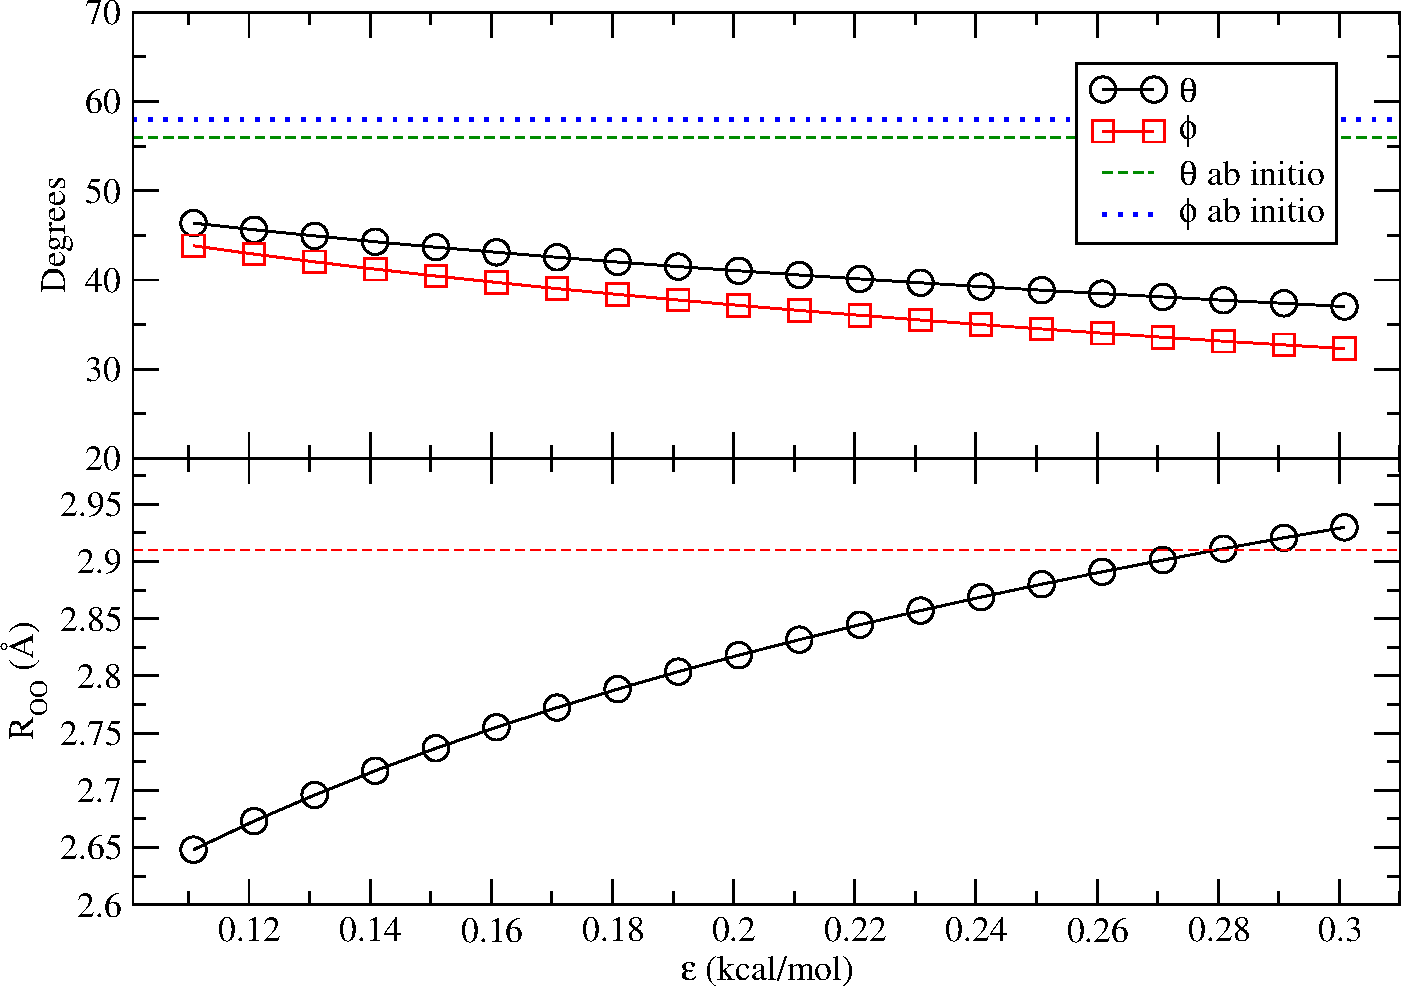
\includegraphics[width = 0.5\textwidth]{Test2_plot.pdf}
\caption{\label{fig:Epsilon} The Lennard-Jones parameter $\epsilon$ was varied while holding the other parameters of the TIP1P/Ice model constant.}
\end{figure}

\subsubsection{Varying Damping $\alpha$}
Having changed both the Lennard-Jones parameters independently and not 
achieving the desired values for the separation distance or angles of the
gas phase water dimer, the next natural parameter of the TIP1P/Ice model to 
vary would be the dipole or quadrupole moment. Before doing so, however, 
we will vary the damping $\alpha$ value which effects how the electrostatics
are calculated in OpenMD\cite{openmd}. In Figure \ref{fig:Dalpha}, we see that
R$_{OO}$ is minimally effected by varying damping $\alpha$ for small values of
$\alpha$. For values larger than about 0.25 \AA$^{-1}$, the dimer separation
distance decreases slighty. However, the ab. initio calculated distance
is not recovered by varying damping $\alpha$ alone. The angles $\theta$ and
$\phi$ also do not converge on the ab. initio predicted values over the range
of damping $\alpha$ investigated here. After talking with Madan, damping
$\alpha$ values of about 0.1 \AA$^{-1}$ are suitable for handling the 
calculation of dipoles and quadrupoles, which is the value that has been used
in all other Tests shown here.

\begin{figure}[h!]
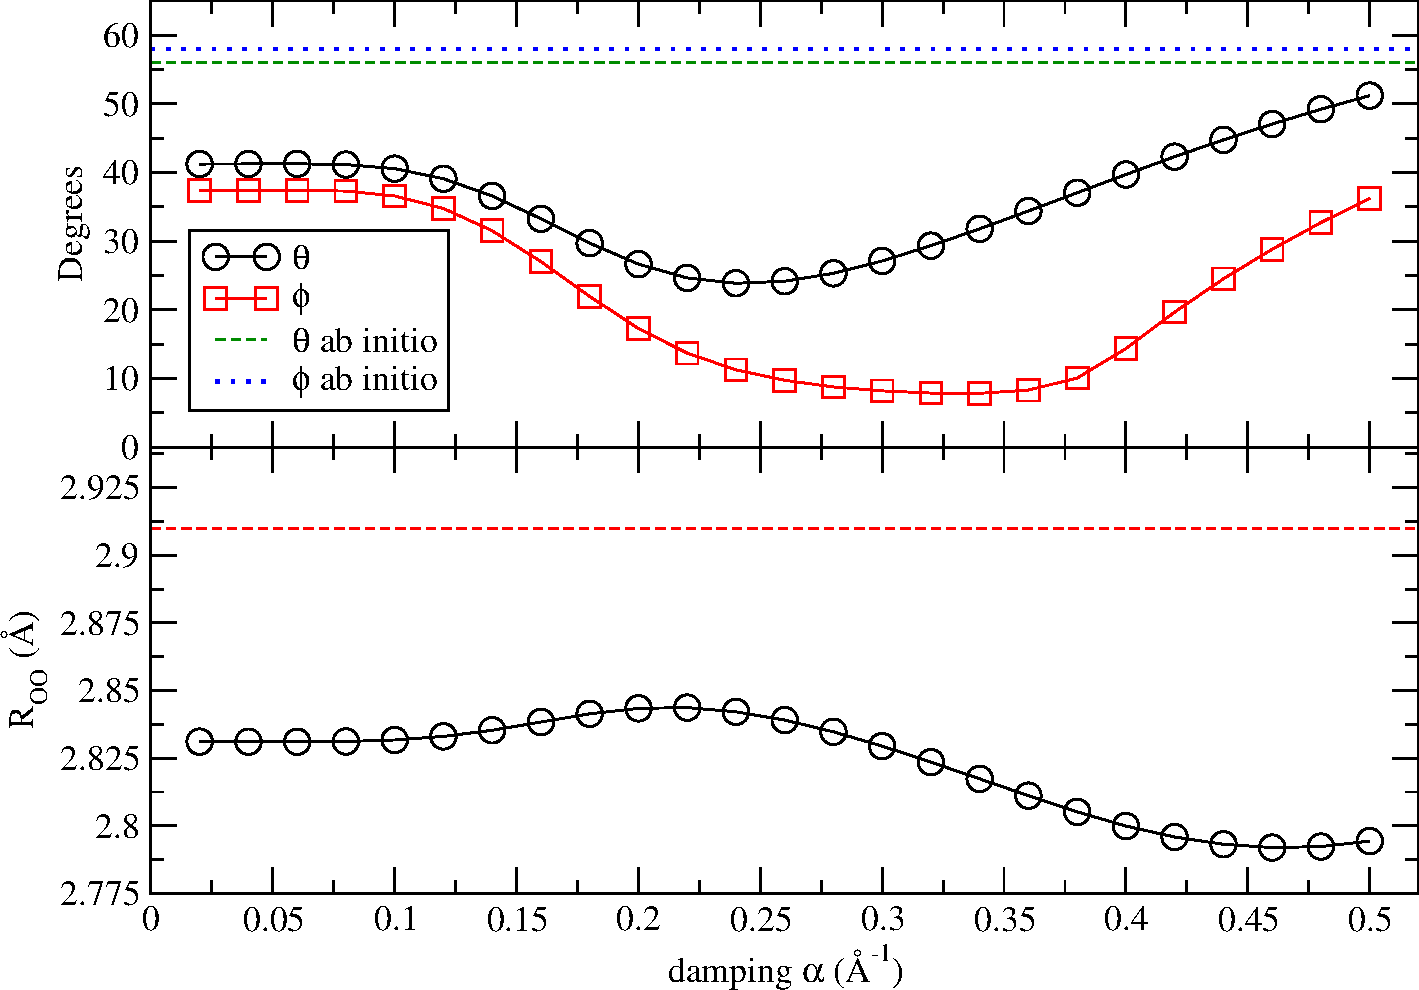
\includegraphics[width = 0.5\textwidth]{Test3_plot.pdf}
\caption{\label{fig:Dalpha} Damping $\alpha$ was varied while holding the otherparameters of the TIP1P/Ice model constant.}
\end{figure}


\subsubsection{Varing the Quadrupole: Introduction of Q$_{xx}$}
A possible reason we have not been able to capture the correct gas phase water
dimer geometry by modifying the Lennard-Jones parameters, may be due to the
initial construction of the quadrupole tensor for the TIP1P/Ice model. In this
model,
as with all planar water models, one of the quadrupole tensor's main diagonal
elements will be zero, given intelligent choice of origin for the coordinate
system. In our construction, this is the Q$_{xx}$ term, as seen in Table
\ref{DQ_Params}. In the following Tests, we will try to incorporate 
the quadrupole moment of the $x$-dimension into our model.

We will consider varying the quadrupole tensor elements of the TIP1P/Ice
model while holding all other parameters constant. This requires special 
consideration though, as we may not want to deviate from TIP1P/Ice's Q$_T$
or $TrQ$ initial values. We initially will consider a Test in which Q$_T$ is 
conserved while varying Q$_{xx}$ by the following constraints. 

\begin{equation}
Q_{yy}^{'} = Q_{yy} + \lambda
\end{equation} 
\begin{equation}
Q_{xx}^{'} = Q_{xx} - \lambda
\end{equation}

While Q$_T$ is conserved in this Test, $TrQ$ is not. In Test 4, seen in Figure
\ref{fig:Qxx}, a similar behavior is apparent as we vary the value of Q$_{xx}$.
Here the $TrQ$ is not conserved, and we have plotted the same data from 
Figure \ref{fig:Qxx} by the $TrQ$ in Figure \ref{fig:Qxx2}. In both graphs,
However, the angle $\phi$ is larger
than $\theta$ at negative values of Q$_{xx}$ here while $\theta$ was larger 
than $\phi$ when we varied Q$_{zz}$. Again no value of Q$_{xx}$ results in the
R$_{OO}$ separation predicted by the ab initio calculations. The angles
also cross over one another as seen previously.  

\begin{figure}[h!]
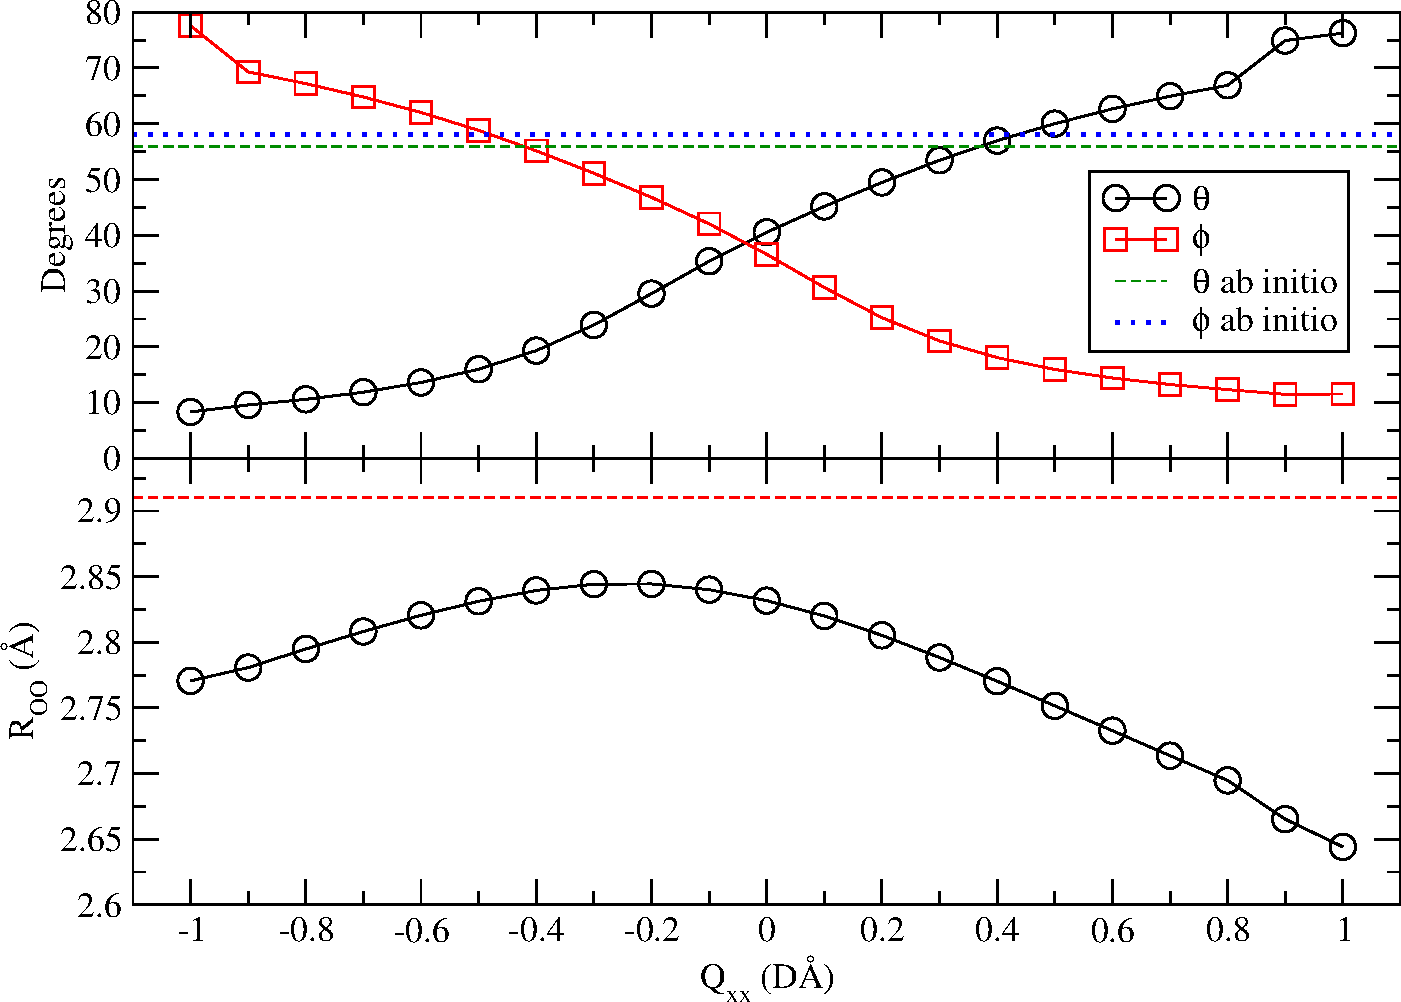
\includegraphics[width = 0.5\textwidth]{Test4_plot.pdf}
\caption{\label{fig:Qxx} The Q$_{xx}$ components of the traced quadrupole tensor were varied while simultaneously adjusting the Q$_{yy}$ component such that the Q$_T$ value for the TIP1P/Ice model was held constant. All other parameters were also held constant and equal to the TIP1P/Ice parameters during this test.This means that $Tr(Q)$ varied since the $Q_{zz}$ component was not adjusted as$Q_{xx}$ was varied.}
\end{figure}


\begin{figure}[h!]
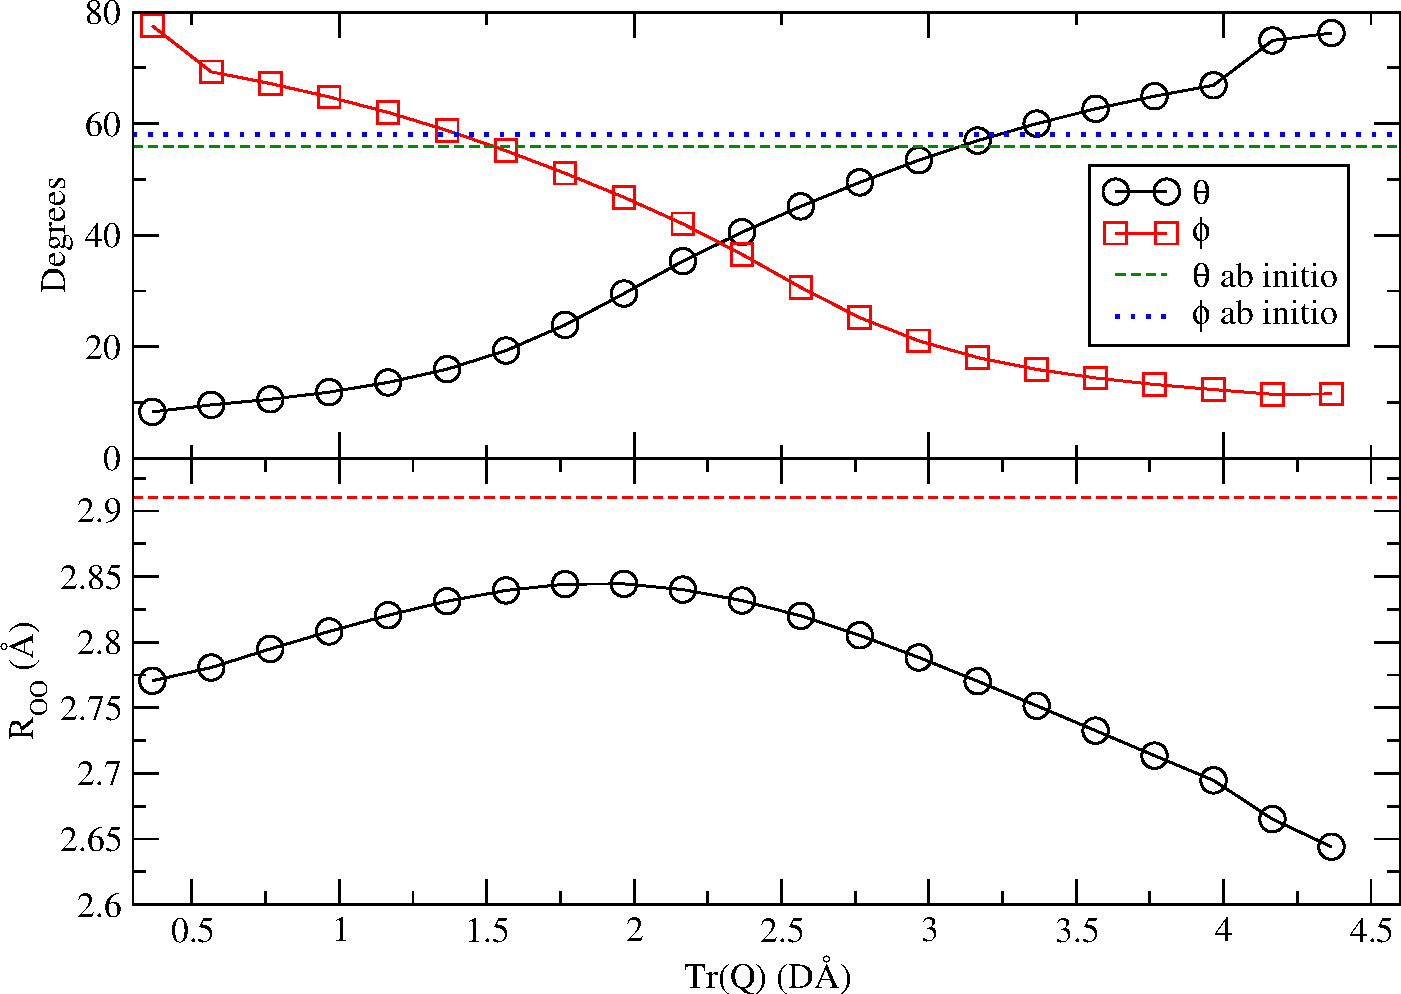
\includegraphics[width = 0.5\textwidth]{Test4_plot2.pdf}
\caption{\label{fig:Qxx2} The same data as plotted in Figure \ref{fig:Qxx}, nowplotted as a function of the $TrQ$.}
\end{figure}

In the next Test, we allow Q$_{xx}$ to vary as in the previous Test, however
we now change Q$_{zz}$ in such a way to keep the $TrQ$ constant to it's 
initial value, as well as varying Q$_{yy}$ in order to conserve Q$_T$. 
In Figure \ref{fig:Qxx3}, we see that the dimer separation 
distance R$_{OO}$ peaks at a Q$_{xx}$ value of about -0.1 D\AA~, and the angles
have the right ordering for which is larger at this value. However, neither 
the R$_{OO}$ or the angles are the correct numerical values as predicted by
the ab initio calculations. Therefore, we will increase the value of 
$\sigma$ to 3.2668 \AA~, determined by the R$_{OO}$ distance in Figure 
\ref{fig:Sigma}. The results of doing so are shown in Figure \ref{fig:Qxx4}. 
Here we see that we have overshot the value of R$_{OO}$, and that our range of
values of Q$_{xx}$ is still quite large. Thus in the next Test, shown in
Figure \ref{fig:Qxx5}, we have adapted a $\sigma$ value of 3.2268 \AA~. Here we
see that we can accurately achieve the correct ordering of the angles, and
approximately 
the correct value for R$_{OO}$ at Q$_{xx}$ values of about -0.02 D\AA~. 

\begin{figure}[h!]
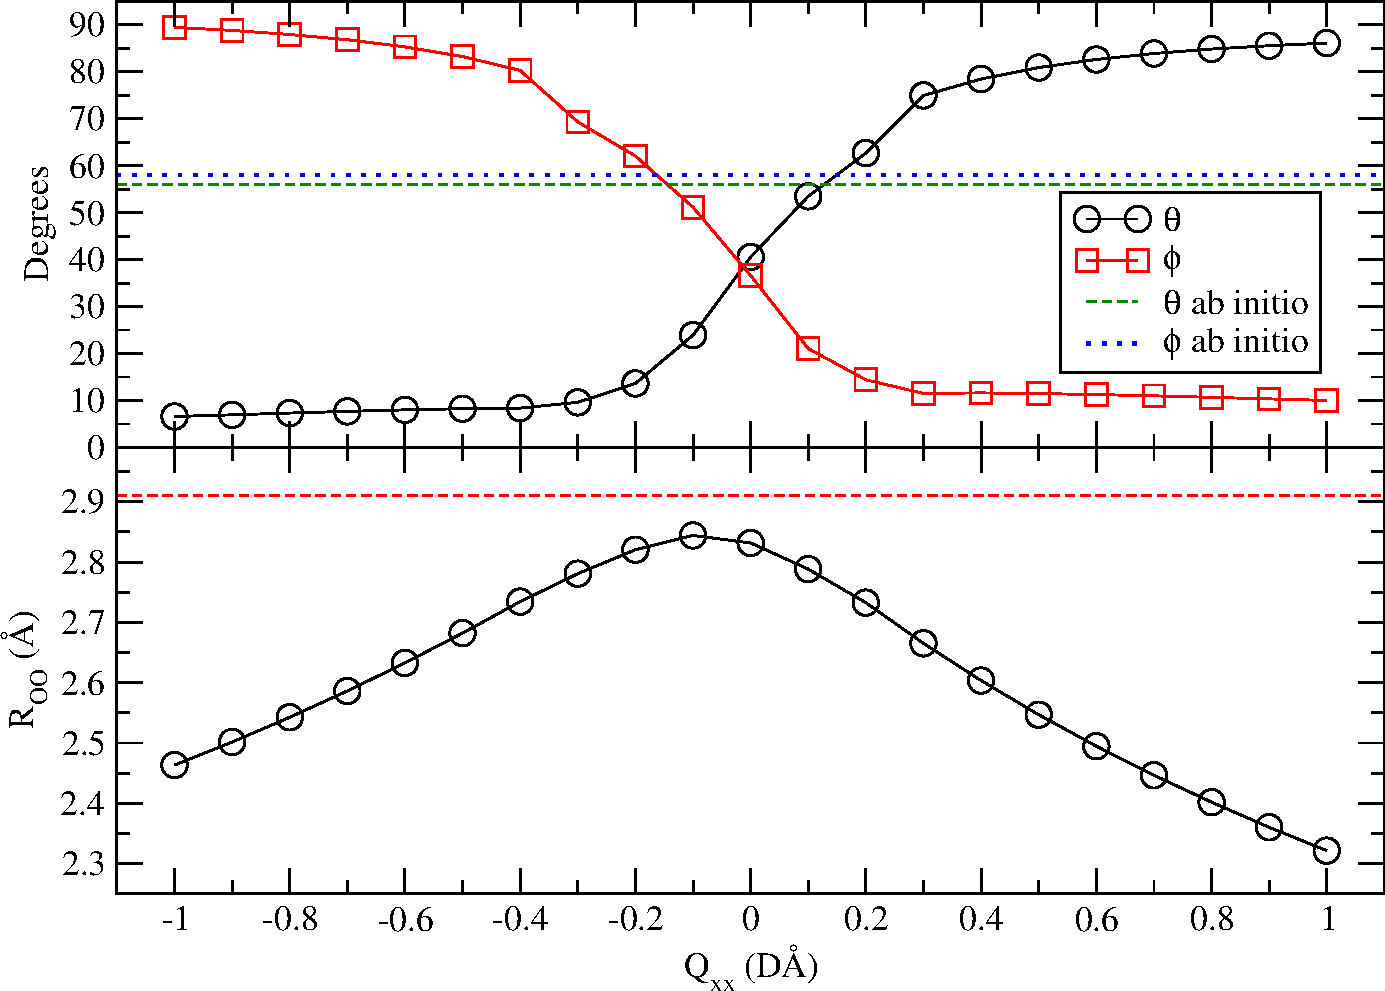
\includegraphics[width = 0.5\textwidth]{Test5_plot.pdf}
\caption{\label{fig:Qxx3} The Q$_{xx}$ components of the traced quadrupole tensor were varied while simultaneously adjusting the Q$_{yy}$ component such that the  Q$_T$ value for the TIP1P/Ice model was held constant. The Q$_{zz}$ component of the quadrupole tensor was also varied in such a way as to keep the $Tr(Q)$ held constant to the TIP1P/Ice value. We see here that the angles cross overone another as in Figure \ref{fig:Qxx}.}
\end{figure}

\begin{figure}[h!]
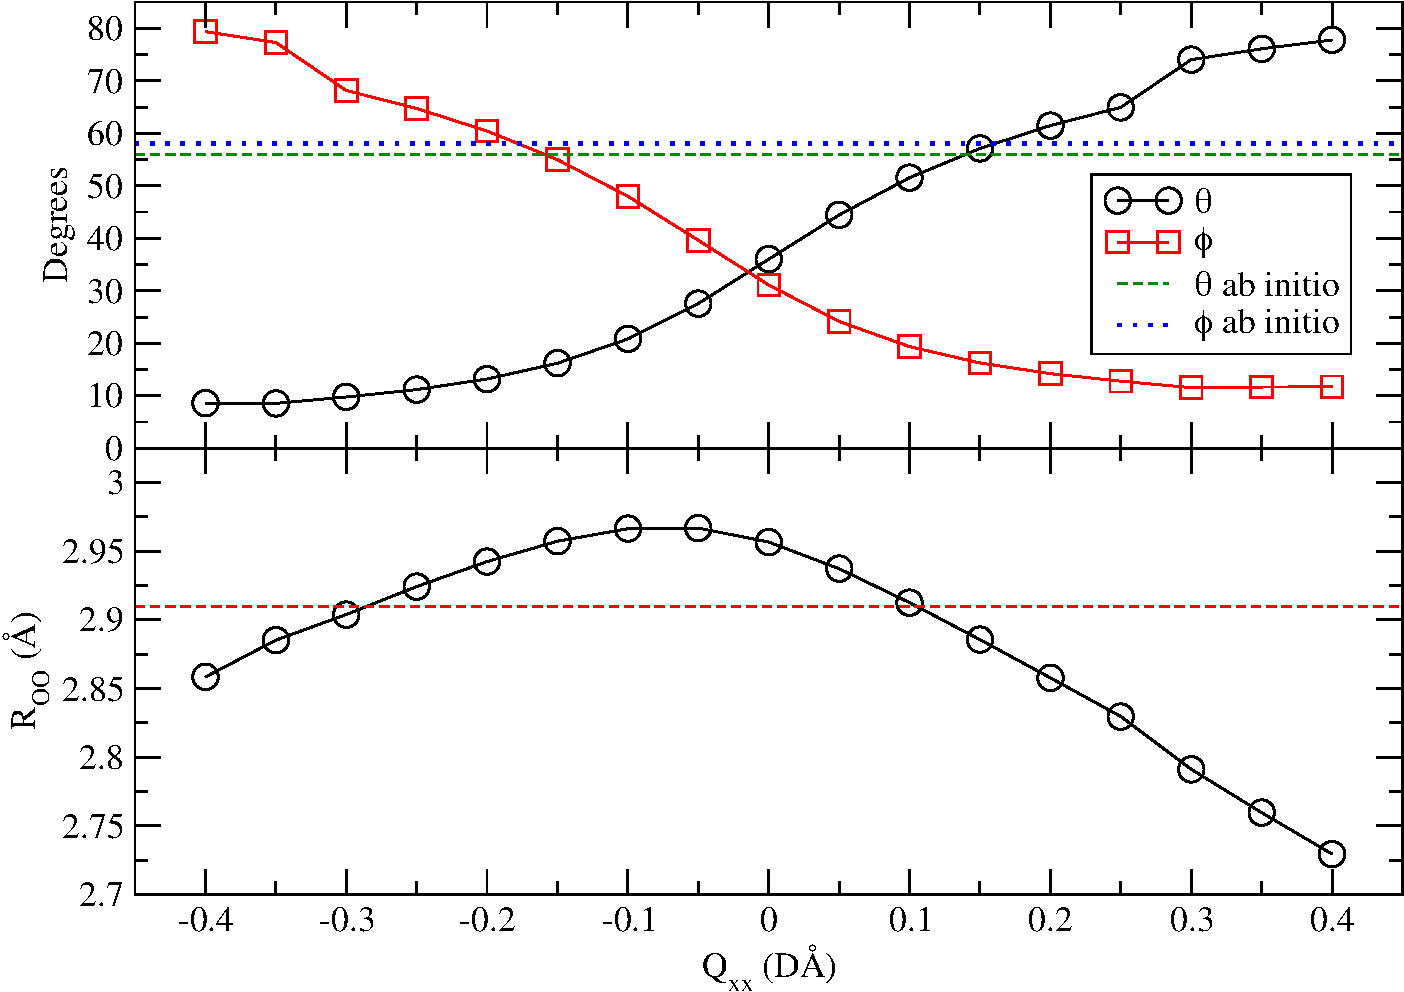
\includegraphics[width = 0.5\textwidth]{Test6_plot.pdf}
\caption{\label{fig:Qxx4} Setting $\sigma$ to 3.2668 \AA~, vary Q$_{xx}$ while simultanesouly adjusting Q$_{yy}$ and Q$_{zz}$ to conserve Q$_T$ and $TrQ$.}
\end{figure}

\begin{figure}[h!]
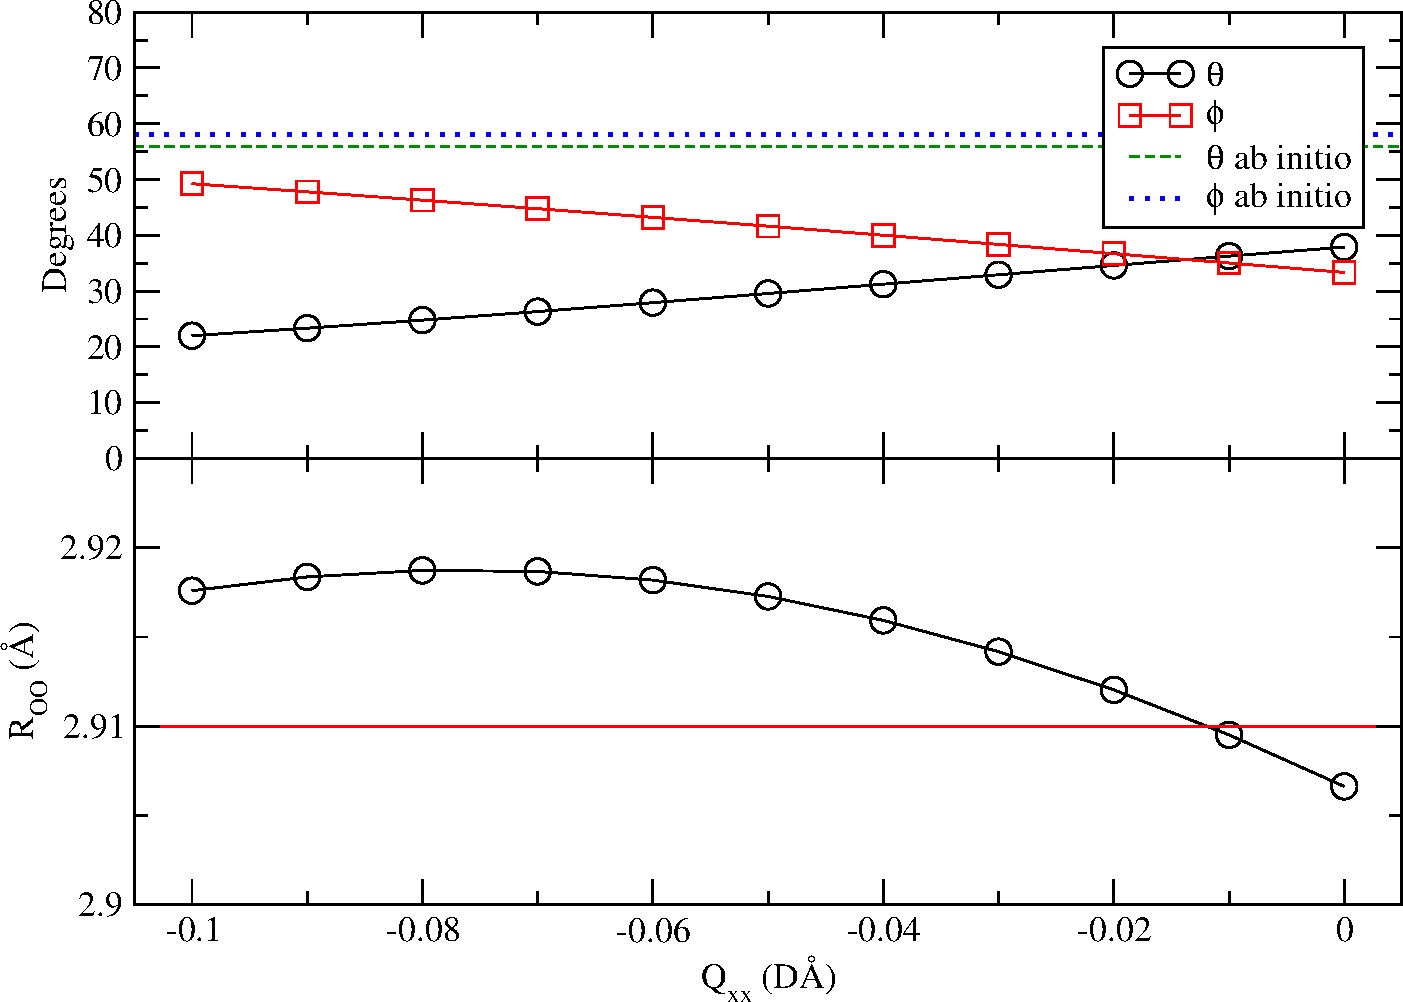
\includegraphics[width = 0.5\textwidth]{Test7_plot.pdf}
\caption{\label{fig:Qxx5} Setting $\sigma$ to 3.2268 \AA~, vary Q$_{xx}$ while simultaneously adjusting Q$_{yy}$ and Q${zz}$ to conserve Q$_T$ and $TrQ$.}
\end{figure}

It appears that we have achieved as close to the ab initio predicted values
as possbile without changing some of our fundamental assumptions. From Figure
\ref{fig:Qxx5}, I believe that by scaling the quadrupole and dipole by 
the same constant, thus keeping their ratio the same, we may be able to achieve
closer agreement with the ab initio predictions. While Abascal and Vega believe
that the largest value of Q$_T$ that will give reasonable T$_m$ for ice I$_h$
to be approximately 2.56 D\AA~, this prediction is made from water models which
contain point charges located on the Hydrogens. These charges cause a torque
on the other water molecule in the dimer structure, resulting in a change of
the magnitude of the angles.

In the following Test, Q$_{xx}$ was varied while simultaneously varying
Q$_{yy}$ to conserve the value of Q$_T$. 
$\mu$ was also scaled by $\mu = 0.996 Q_T$ for each Q$_T$ investigated. 
The $TrQ$ was set to 2.365707 D\AA~, and $\sigma$
was set to 3.2268 \AA~. In Figure \ref{fig:Q_T},R$_{OO}$, $\theta$, and 
$\phi$ are shown as Q$_{xx}$ and Q$_{yy}$ are varied.

\begin{figure}[h!]
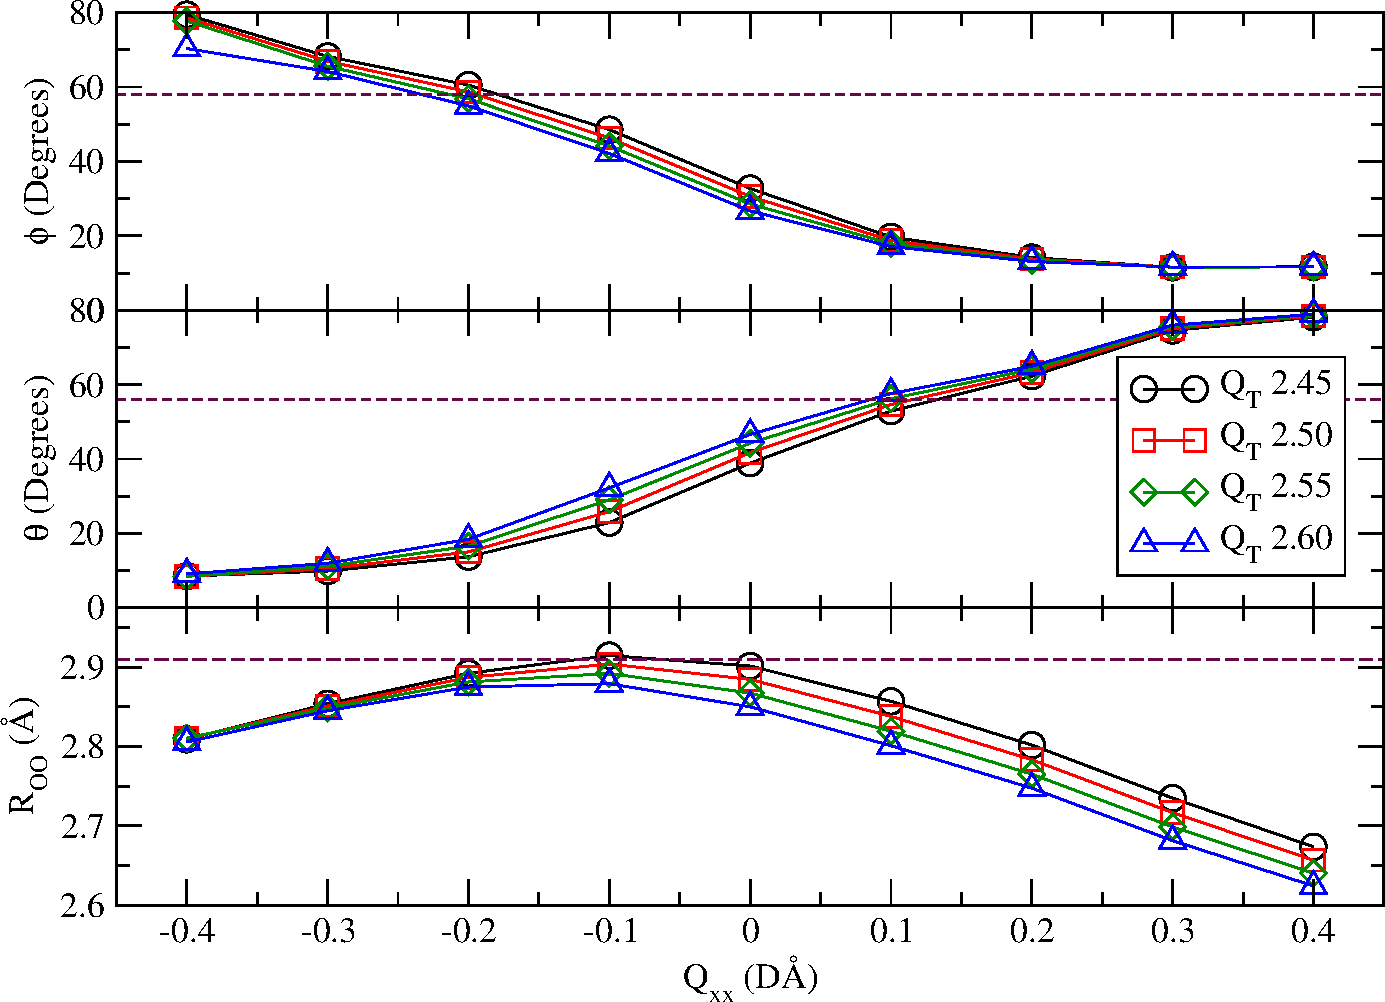
\includegraphics[width=0.5\textwidth]{Test12_plot.pdf}
\caption{\label{fig:Q_T}Here Q$_{xx}$ and Q$_{yy}$ are varied simulatneously to conserve the value of Q$_T$. $\mu$ is scaled as $0.996 Q_T$, thus the ratio of $\mu$ to Q$_T$ is conserved for each Test of Q$_T$. The $TrQ$ is fixed to a set value, thus Q$_{zz}$ varies as the other components do. }
\end{figure}


In the next Test, the dipole moment of the model was varied by some scalar
amount ($\lambda$), relative to the Q$_T$ chosen. The Q$_{xx}$ component
of the quadrupole tensor was set to null, so Q$_{yy}$ varied for each 
case of Q$_T$. Q$_{zz}$ was fixed to the TIP1P/Ice model's value. The
results of this test can be seen in Figure \ref{fig:mew}.

\begin{figure}[h!]
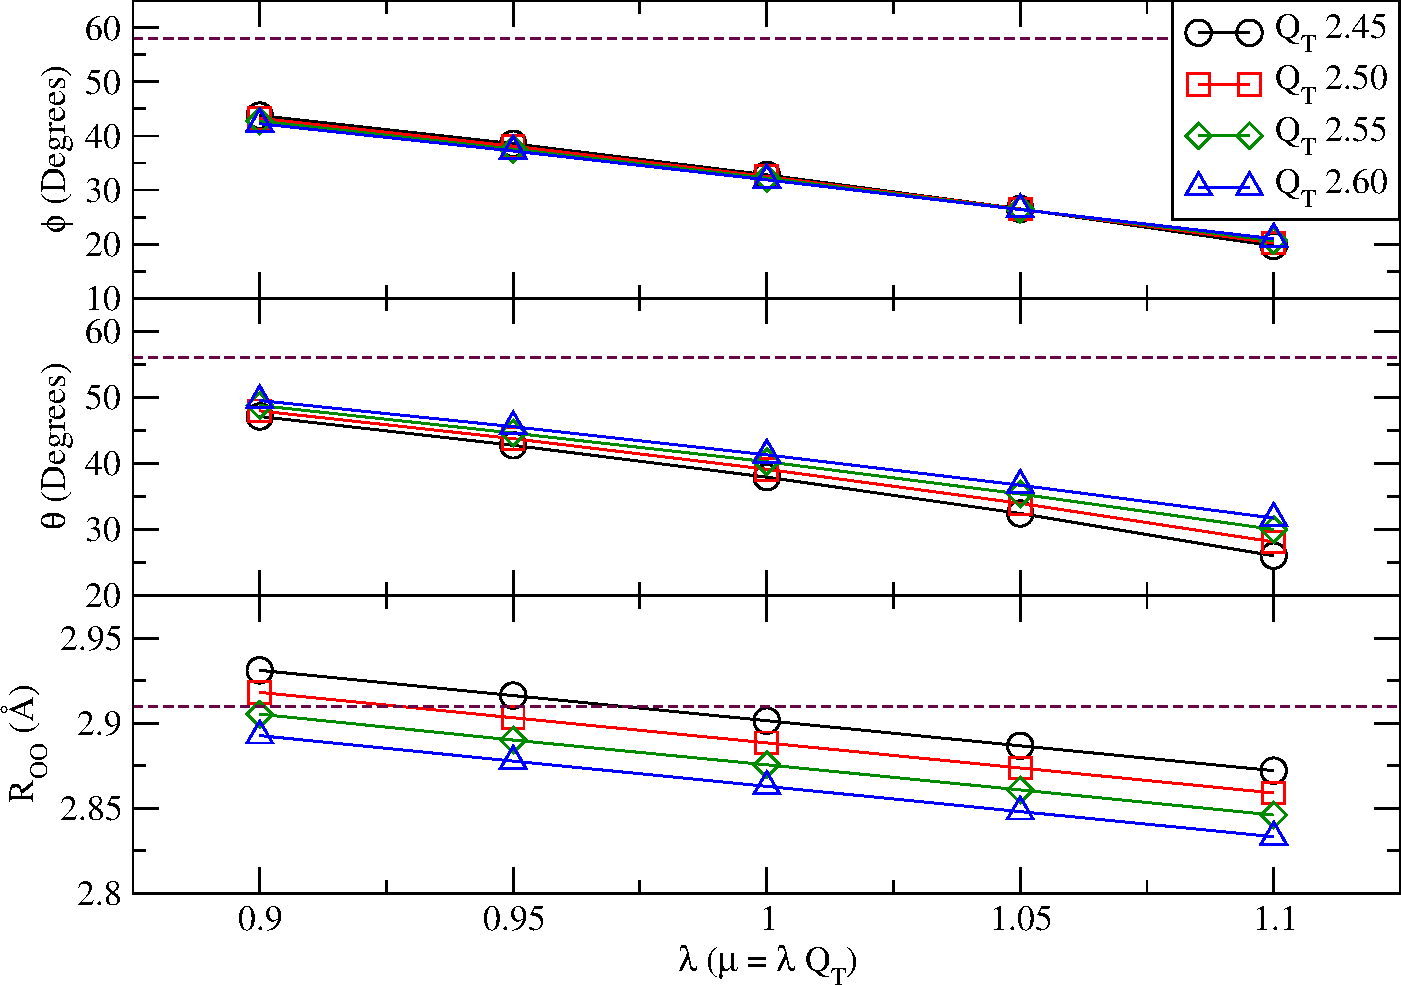
\includegraphics[width=0.5\textwidth]{Test16_plot.pdf}
\caption{\label{fig:mew} }
\end{figure}
In the next section, I will construct a water model similar to the TIP1P/Ice 
model, however, it will not be the result of collapsing a many-site model onto
a single-site. This model will be derived from the results shown in this 
section with a larger dipole and quadrupole, in attempts to increase the 
magnitude of both of the angles without obscuring their ordering or the 
R$_{OO}$ values obtained above.

\subsection{TIP1P/Ice 2.0}

%The starting parameters for this section will be as follows: $\sigma = 3.2268$
%\AA~, $\mu = 2.56$ D, Q$_T = 2.56$, and the rest of the parameters are set to 
%the previous values.

%In Test 1, we will vary Q$_{xx}$ and Q$_{yy}$ while holding Q$_T$ constant. 
%Q$_{zz}$ is chosen to be a constant 0.73 D \AA~, thus the $TrQ$ will vary 
%throughout Test 1. In Figure \ref{fig:Qxx6}, R$_{OO}$ does not achieve the 
%ab initio predicted value of 2.91 \AA~, though comes closest at Q$_{xx}$
%values of about -0.3 D\AA~. 

%\begin{figure}[h!]
%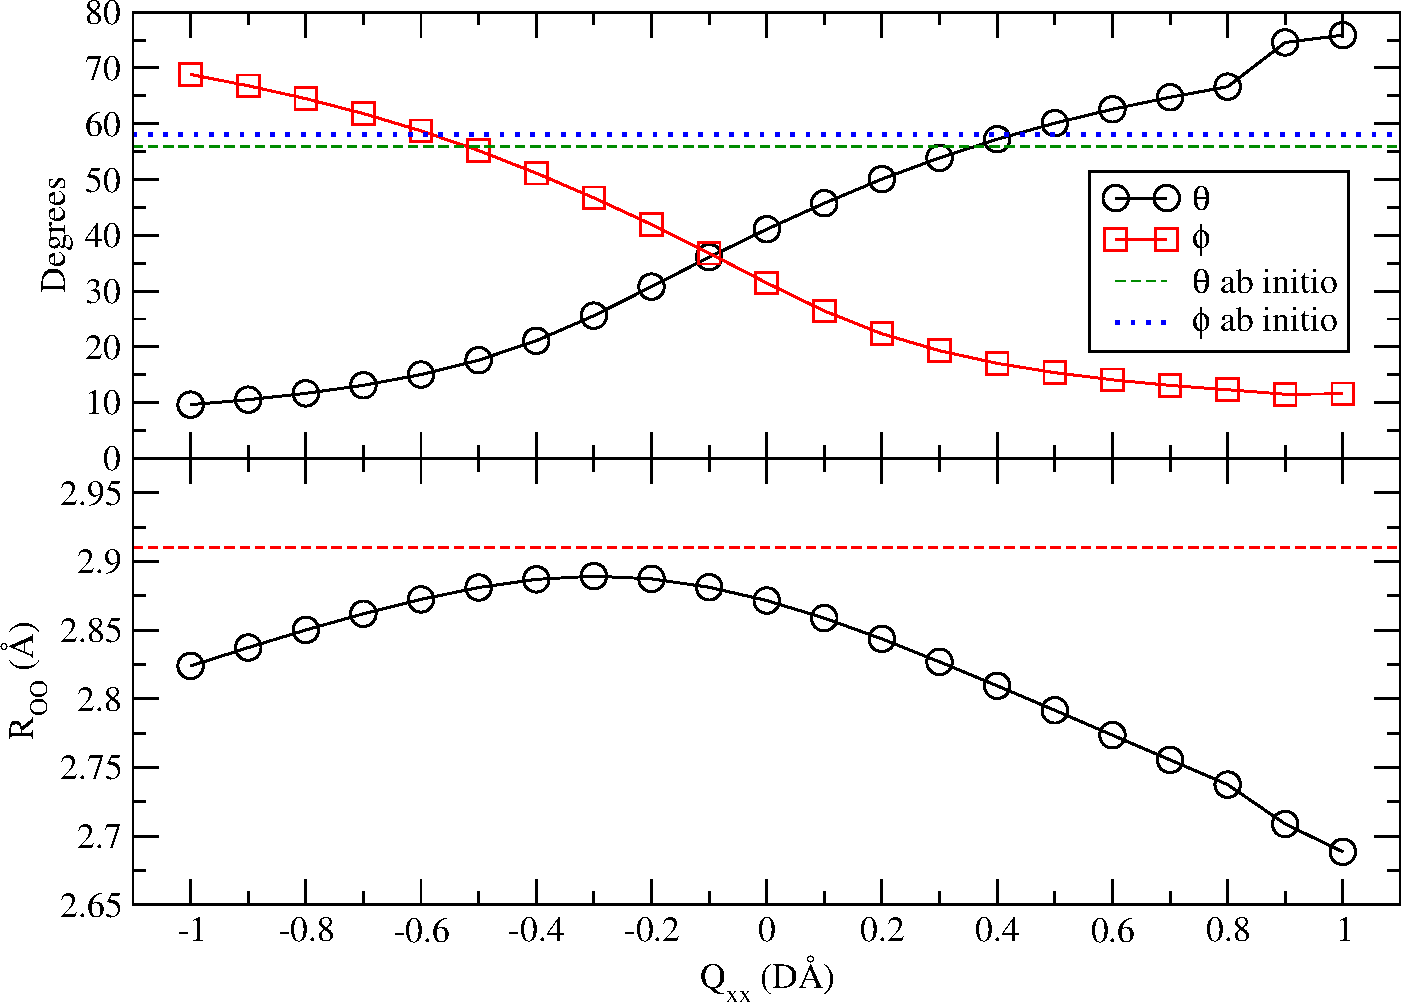
\includegraphics[width = 0.5\textwidth]{Test8_plot.pdf}
%\caption{\label{fig:Qxx6}Q$_{xx}$ is varied while simultaneously adjusting Q$_{yy}$ so that Q$_T$ is conserved. Q$_{zz}$ is not varied here, so the $TrQ$ changes as Q$_{xx}$ changes.}
%\end{figure}

In this section, we will worry less about holding Q$_T$ constant, and instead
hold QBar constant. In Figure \ref{fig:Qyy}, we have the results of varying
Q$_{yy}$ while holding Q$_{xx}$ constant at 0.1 D\AA~, and varying Q$_{zz}$
such that QBar fixed at the TIP4P/Ice value. However, we see that we do
not recover the TIP4P/Ice water dimer geometry.

\begin{figure}[h!]
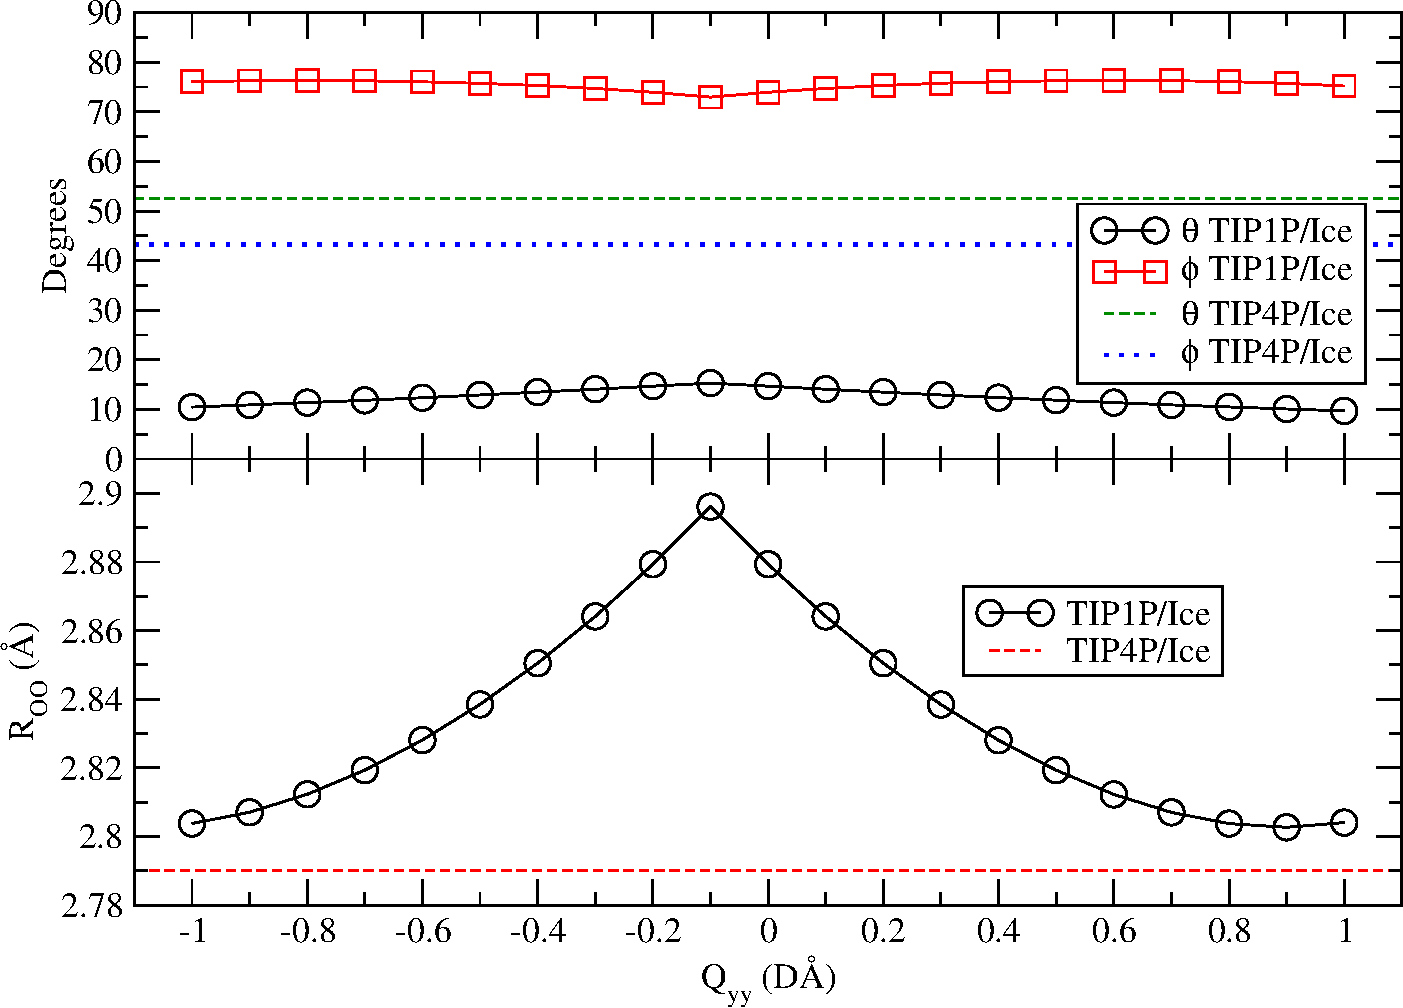
\includegraphics[width=0.5\textwidth]{Test19_plot.pdf}
\caption{\label{fig:Qyy} Q$_{xx} = -0.1$, QBar set to the TIP4P/Ice QBar value of $2.8141$, Q$_{zz}$ was modified to keep this constant as Q$_{yy}$ changed.}
\end{figure}

It is interesting to note that the value of $\phi$ in Figure \ref{fig:Qyy} is 
much greater than initially expected from Figure \ref{fig:Qxx}. There, we would
predict $\phi \approx 40$ degrees, while here we have obtained a value of about
$76$ degrees. Also, there does not appear to be any appreciable change in the
values of $\theta$ as we vary Q$_{yy}$. This makes me wonder what controls
the value of $\theta$, as it appears to not be the value of Q$_{yy}$ as 
initially thought. In Figure \ref{fig:Qyy2}, we have held Q$_{yy}$ constant
at -0.1 D\AA~, and varied Q$_{xx}$ to see if it controls both $\phi$ and
$\theta$.

\begin{figure}[h!]
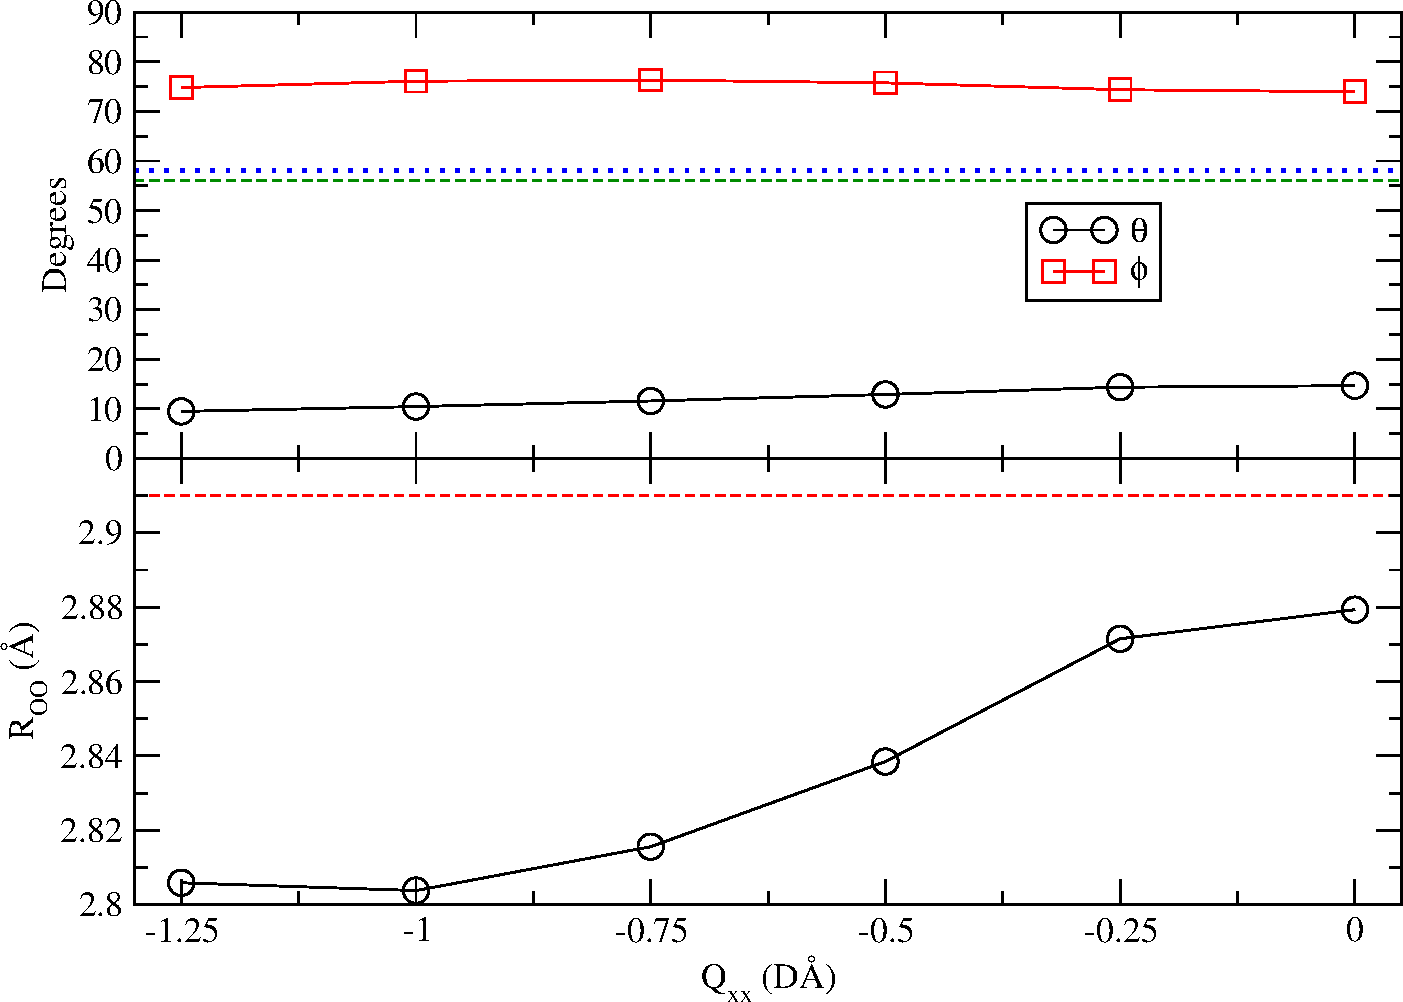
\includegraphics[width=0.5\textwidth]{Test20_plot.pdf}
\caption{\label{fig:Qyy2} Q$_{yy} = -0.1$, Q$_{zz}$ was varied to keep QBar constant and equal to the TIP4P/Ice model's value of 2.8141.}
\end{figure}

From Figure \ref{fig:Qyy2}, we see that while R$_{OO}$ is slightly sensative
to the value of Q$_{xx}$, the angles $\theta$ and $\phi$ are both insensative
to it. In order to try and understand if and how the angles are dependent
on QBar, I have re-plotted the data from Figure \ref{fig:Qxx3} as a function
of QBar instead of Q$_{xx}$. This can be seen in Figure \ref{fig:QBar2}.

\begin{figure}[h!]
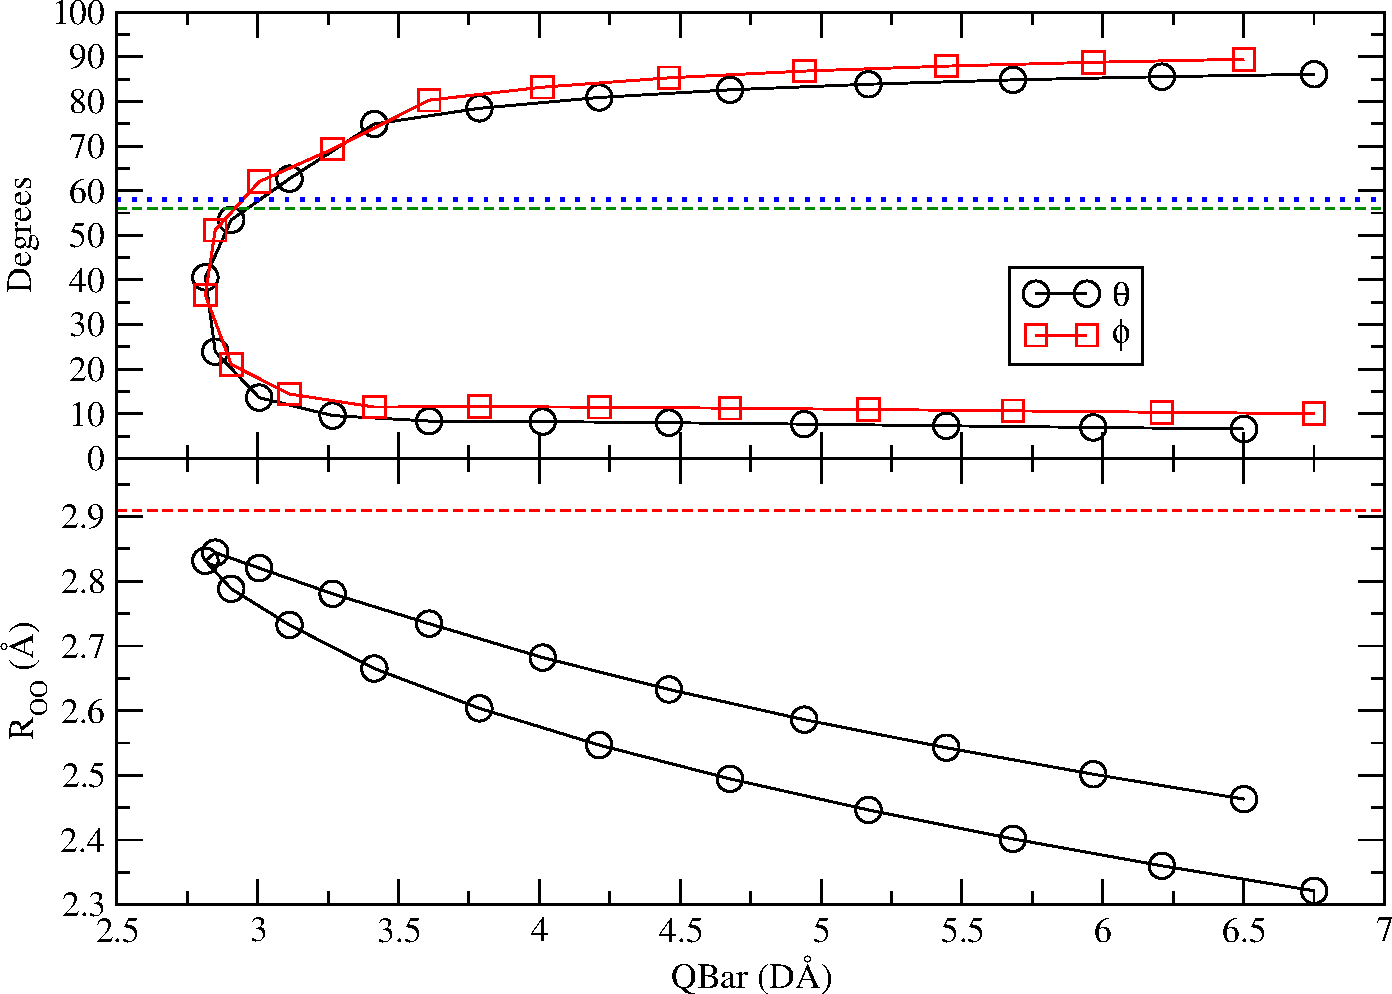
\includegraphics[width=0.5\textwidth]{Test5_plot2.pdf}
\caption{\label{fig:QBar2}Q$_{xx}$ and Q$_{yy}$ varied while holding Q$_T$ constant, Q$_{zz}$ varied in order to keep $TrQ$ constant. Both Q$_T$ and $TrQ$ were set to the TIP4P/Ice model value.}
\end{figure} 

An interesting follow up test will be 
to set Q$_{xx}$ and Q$_{yy}$ to -0.1, Q$_{zz}$ to 1.3071, and vary $\mu$ to 
see if the desired angles can be achieved with a smaller dipole moment. The
results of doing so are shown in Figure \ref{fig:mu2}.

\begin{figure}[h!]
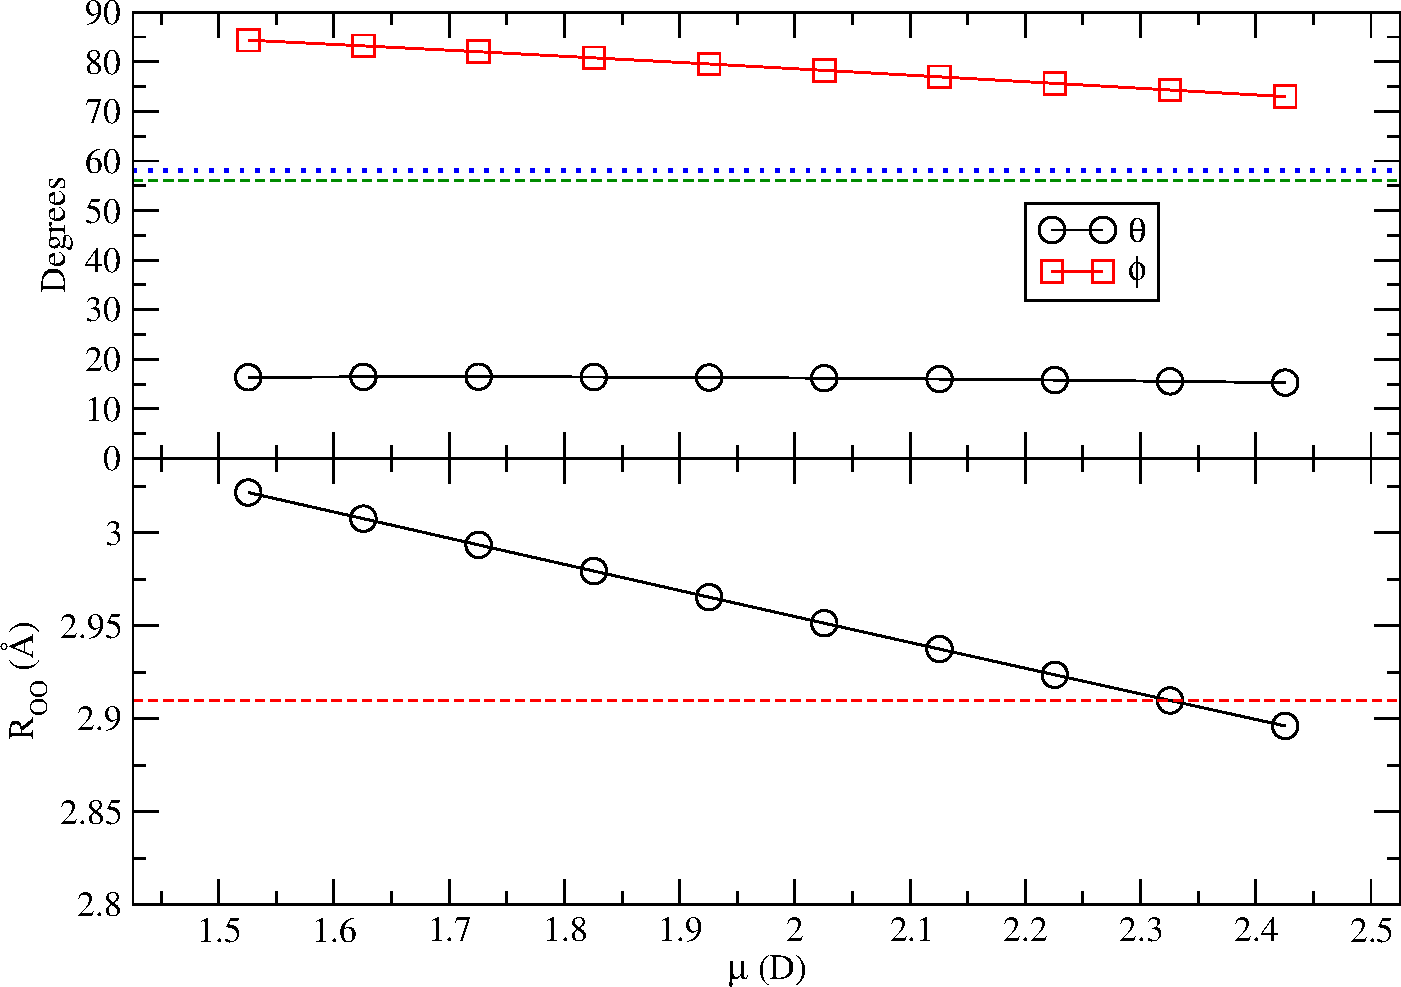
\includegraphics[width=0.5\textwidth]{Test22_plot.pdf}
\caption{\label{fig:mu2} Q$_{xx} = -0.1$, Q$_{yy} = -0.1$, Q$_{zz} = 1.3701$ which ensures QBar is set to the TIP4P/Ice model value of $2.8141$ D\AA~.}
\end{figure}

In Figure \ref{fig:mu2}, we see that as we decrease the value of the dipole 
moment, the water dimer's separation distance, R$_{OO}$ gradually becomes 
larger. The angle $\phi$ increases slightly with decreasing $\mu$, however, 
$\theta$ is relatively insensitive to the value of $\mu$.
 
In the next Test, we have set the Lennard-Jones parameters to that of the
TIP4P/Ice model, as well as the Q$_{xx}$ and Q${zz}$ values. Q$_{yy}$ is 
allowed to vary, and as such, Q$_T$ and QBar both vary. In Figure
\ref{fig:Qyy3}, we see that the angle $\theta$ is obtained when Q$_{yy}$
is set to about 1.87 D\AA~. However, we see that we miss the dimer 
separation distance at this value of Q$_{yy}$, as well as the angle
$\phi$, which we believe to be the less important of the two angles.

\begin{figure}[h!]
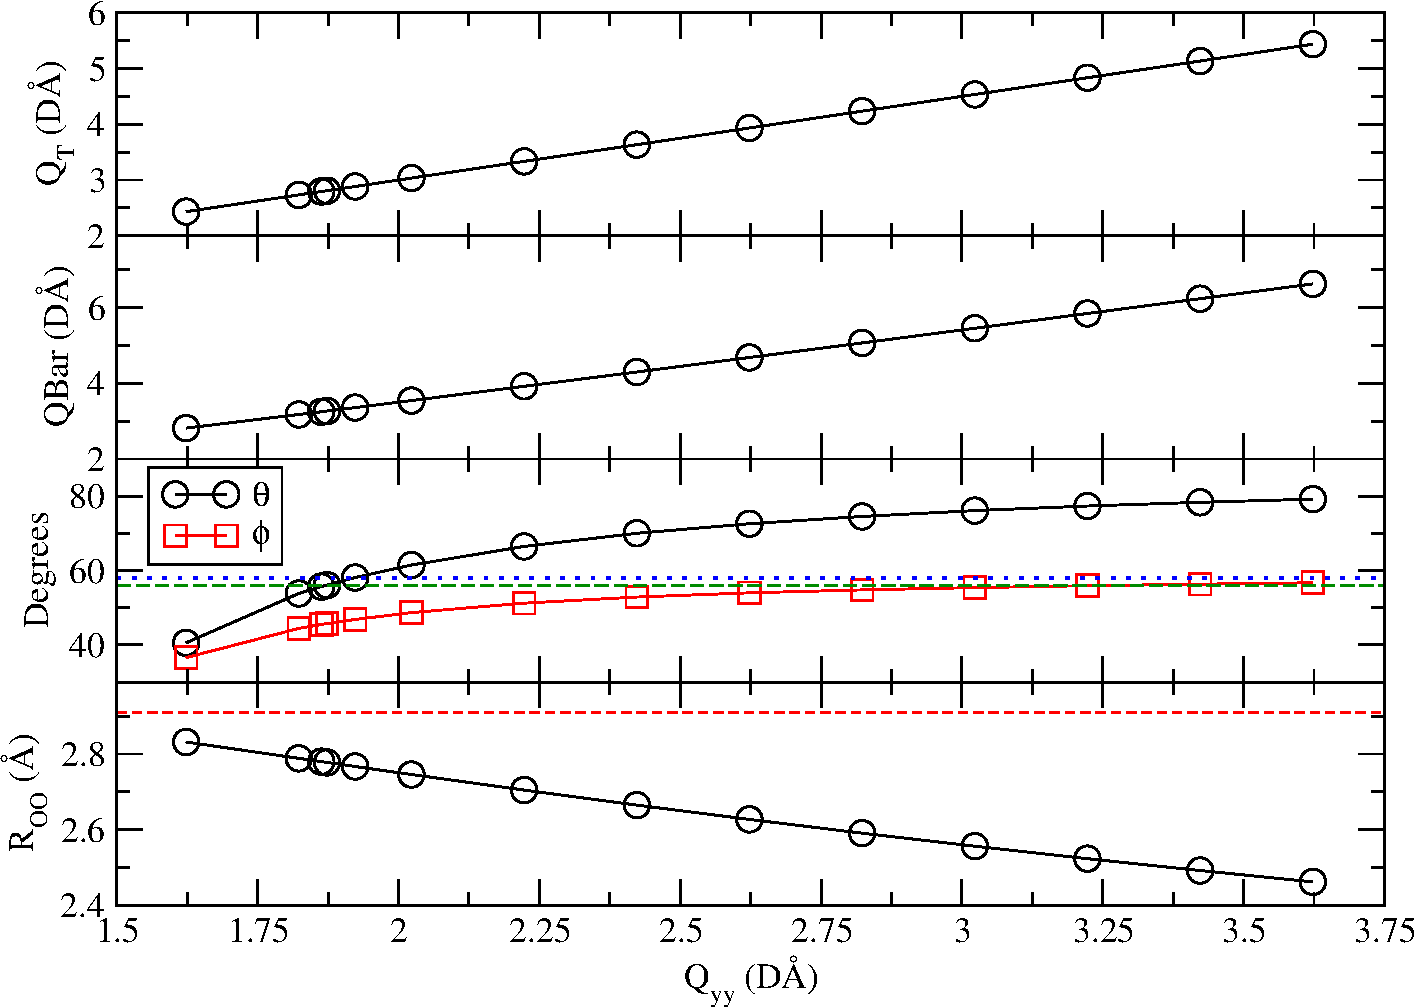
\includegraphics[width=0.5\textwidth]{Test23_plot.pdf}
\caption{\label{fig:Qyy3} Q$_{xx}$ and Q$_{zz}$ are set to the TIP4P/Ice value, as well as the Lennard-Jones parameters.The left most data point is the parameter set of the TIP4P/Ice model.}
\end{figure}

In a similar way, we have held Q$_{yy}$ and Q$_{zz}$ constant while varying
Q$_{xx}$. The results of doing so can be seen in Figure \ref{fig:Qyy4}.

\begin{figure}[h!]
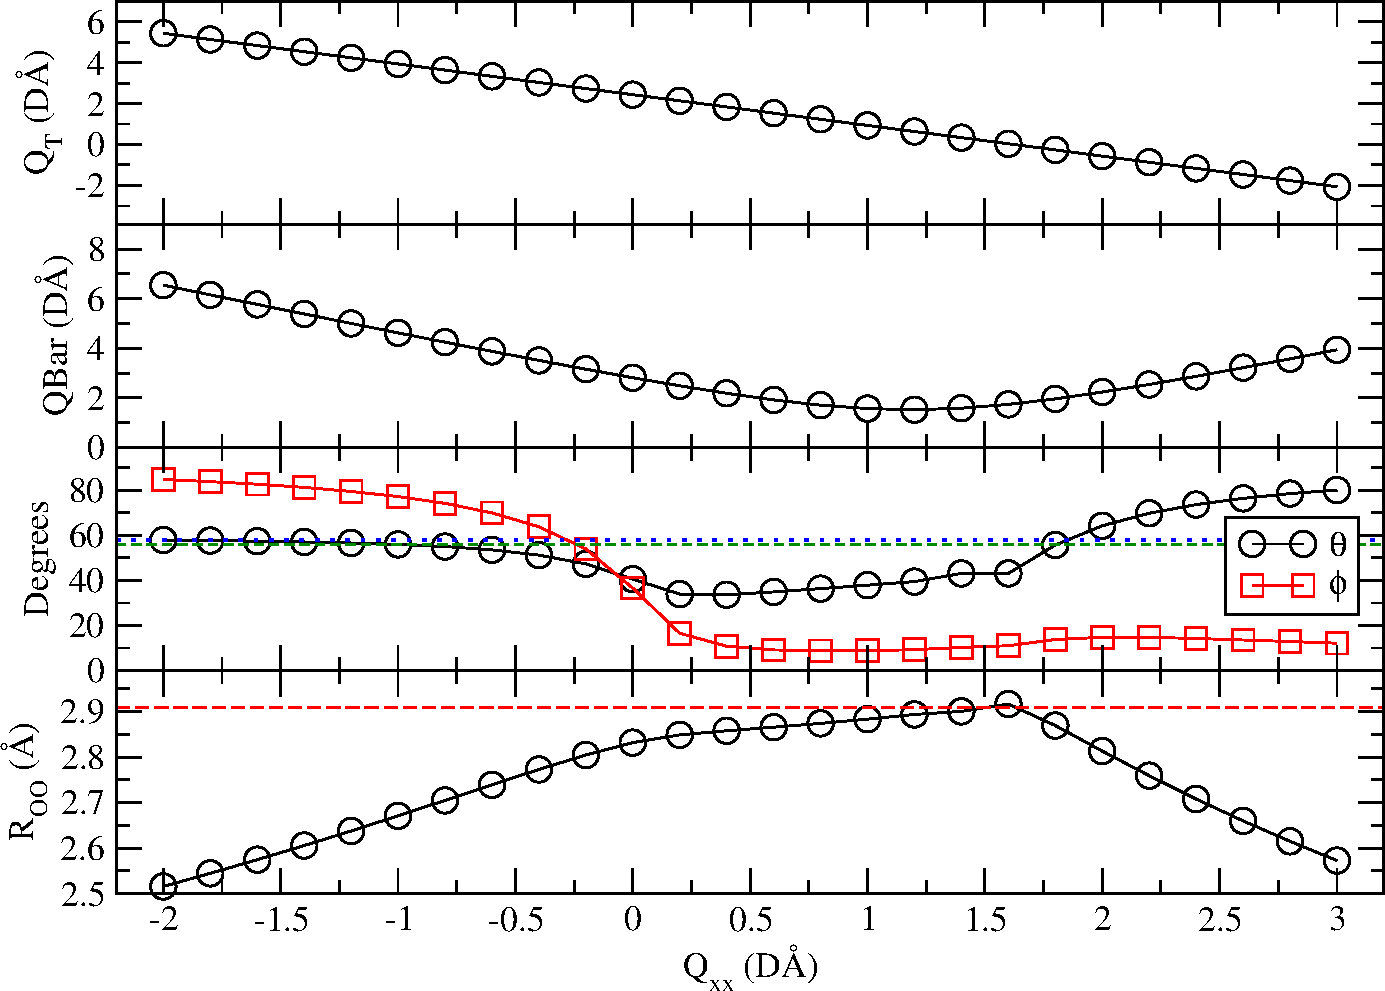
\includegraphics[width=0.5\textwidth]{Test24_plot.pdf}
\caption{\label{fig:Qyy4} Q$_{yy}$ and Q$_{zz}$ are set to the TIP4P/Ice value,as well as the Lennard-Jones parameters.The left most data point is the parameter set of the TIP4P/Ice model.}
\end{figure}

Finally, we have finished the permutation by varying Q$_{zz}$ while holding
Q$_{xx}$ and Q${yy}$ constant at their original TIP4P/Ice values, as seen
in Figure \ref{fig:Qyy5}.

\begin{figure}[h!]
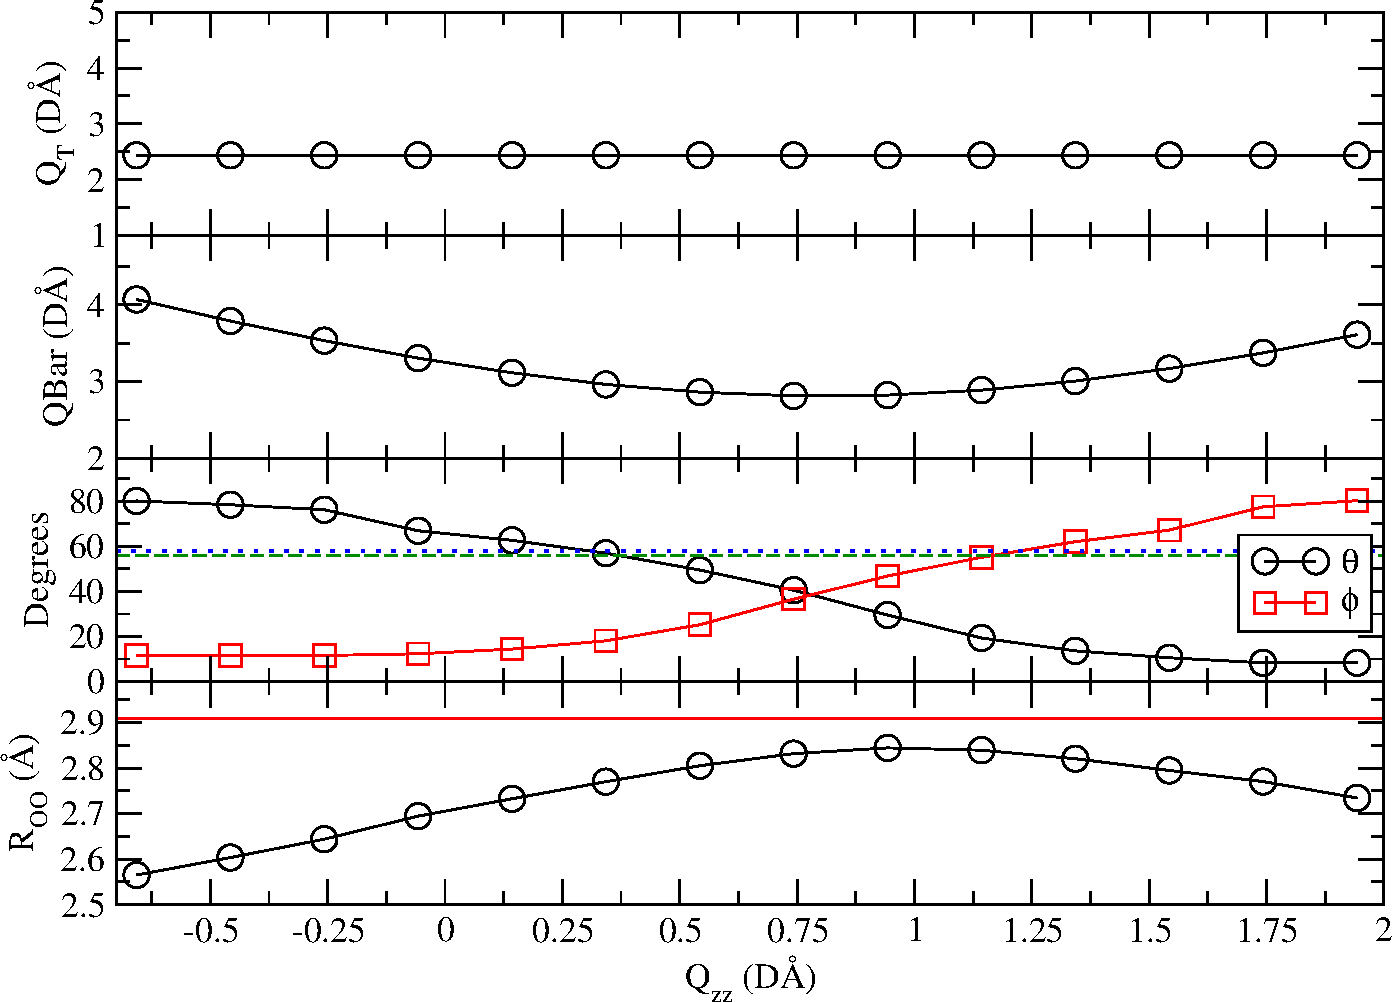
\includegraphics[width=0.5\textwidth]{Test25_plot.pdf}
\caption{\label{fig:Qyy5} Q$_{xx}$ and Q$_{yy}$ are set to the TIP4P/Ice value,\
as well as the Lennard-Jones parameters.The left most data point is the parameter set of the TIP4P/Ice model.}
\end{figure}


\subsection{Bulk Properties}
As an initial test of the bulk phase properties, I have equilibrated two
separate water boxes, one containing 1372 molecules, and one
containing 4000 molecules. The resulting geometry was a cubic
box with side length of 48.57617 \AA~. The molecules were propaged at 300K for
1 nanosecond, saving coordinates every 0.1 ps for analysis. The 
three-dimensional diffusion constant was found to be 
$5.488\times10^{-5}$cm$^{2}$s$^{-1}$. This is about a factor of two larger
than the experimentally reported value of 2.30 cm$^{2}$s$^{-1}$. We attribute
this difference to a lack of strength of hydrogen bonding. Due to this,
we will try playing with the dipole strength and the Q$_{zz}$ values.
		

\subsection{Basal Ice I$_{h}$/water Coexistence}
In order to tune the model to the desired observable, I have begun testing 
the model at the ice I$_{h}$/water interface, exposing a basal plane to bulk 
water. This system was prepared by constructing a large block of ice from 
crystallographic coordinates taken from Hirsch and Ojamae structure number
6\cite{Hirsch04}. The constructed block is periodic in all three dimensions. 
The block was positioned in a simulation cell such that the basal face pointed
along the positive $z$-dimension. The ice block was allowed to relax and 
equilibrated to 75 K. Separately, a simulation box of liquid water with a 
density of 0.999 g cm$^{-1}$ was 
equilibrated to 75 K, with equivalent $x$ and $y$ dimensions to the ice block,
and twice that in $z$. The ice block was then merged with the liquid system
by carving out any liquid water molecule within three angstroms of a molecule
from the ice system.
	
%		\caption{\label{fig:RC} Comparison of ``Bragg Peak" location at 0.1 T and 0.2 T on the (111) symmetry axis.  It would appear that the Bragg peak is actually background fluctuations, and that the initial location at the correct $\vec{q}$ was an unfortunate coincidence.}
%	\end{figure}
	
%	\begin{figure}
%		\includegraphics[width=0.45\textwidth]{fwhm.pdf}
%		\caption{\label{fig:fwhm} Comparison of ``Bragg Peak" location at 0.1 T and 0.2 T on the (111) symmetry axis.  It would appear that the Bragg peak is actually background fluctuations, and that the initial location at the correct $\vec{q}$ was an unfortunate coincidence.}
%	\end{figure}

		


\section{Conclusions}
In conclusion, we have not yet found an accurate model.

		%\caption{\label{fig:fwhm} Comparison of ``Bragg Peak" location at 0.1 T and 0.2 T on the (111) symmetry axis.  It would appear that the Bragg peak is actually background fluctuations, and that the initial location at the correct $\vec{q}$ was an unfortunate coincidence.}


%\bibliographystyle{apsrev}
\bibliographystyle{aip}
\bibliography{iceWater}
%\begin{thebibliography}{widestentry}
%\end{thebibliography}

\end{document}
